\documentclass[a4paper, 11pt]{report}
\usepackage[utf8]{inputenc}
\usepackage{amsmath,tabto}
\usepackage[hidelinks]{hyperref}
\usepackage{titlesec}
\titleformat{\chapter}[display]
  {\normalfont\bfseries}{}{0pt}{\Huge}
\usepackage{graphicx}
\usepackage{subcaption}
\usepackage{caption}
\usepackage{glossaries}
\graphicspath{ {images/} }
\date{null}
\usepackage{fullpage} % changes the margin
\usepackage{setspace}
\usepackage{multirow}

\begin{document}
\begin{titlepage} % Suppresses displaying the page number on the title page and the subsequent page counts as page 1
	\newcommand{\HRule}{\rule{\linewidth}{0.5mm}} % Defines a new command for horizontal lines, change thickness here
	
	\center % Centre everything on the page
	
	%------------------------------------------------
	%	Headings
	%------------------------------------------------
	
	\textsc{\LARGE Concordia University}\\[1.5cm] % Main heading such as the name of your university/college
	

	%------------------------------------------------
	%	Title
	%------------------------------------------------
	
	\HRule\\[0.4cm]
	
	{\huge\bfseries  SOEN 6481 - Software Design  Methodologies}\\[0.4cm] % Title of your document
	
	\HRule\\[1.5cm]
	\textsc{\Large Deliverable 2}\\[0.5cm] % Major heading such as course name
	\textsc{\Large Requirement Analysis for Ticket Vending Machine}\\[0.5cm]
	%------------------------------------------------
	%	Author(s)
	%------------------------------------------------
	
% 	\begin{minipage}{0.4\textwidth}
% 		\begin{flushleft}
			
% 			\end{flushleft}
% 	\end{minipage}
	~
% 	\begin{minipage}{0.4\textwidth}
% 		\begin{flushright}
			\large
			\textit{Supervisor}\\
			Prof. Pankaj Kamthan\\[0.5cm] % Supervisor's name
% 		\end{flushright}
% 	\end{minipage}
    \vfill
    \large
            \textbf{Team K}\\
			\textit{Authors}\\
		Devanshi Piyushkumar Patel - \textsc{40172139}\\
            Hetul Patel - \textsc{40225667}\\
            Jay Bharatbhai Patel - \textsc{40197003}\\
            Juhi Birju Patel - \textsc{40190446}\\
            Krishna Patel - \textsc {40206701}\\
            Mahavir Patel - \textsc {40198619}\\[0.75cm]
            
	
	% If you don't want a supervisor, uncomment the two lines below and comment the code above
	%{\large\textit{Author}}\\
	%John \textsc{Smith} % Your name
	
	%------------------------------------------------
	%	Date
	%------------------------------------------------
	
	\vfill\vfill\vfill\vfill% Position the date 3/4 down the remaining page
	\textbf{GitHub Address:} \url{https://github.com/mahavir0/iGo---SOEN-6461-SDM}

	%------------------------------------------------
	%	Logo
	%------------------------------------------------
	
 	\vfill\vfill
 	
\includegraphics[scale=0.5]{concordia-logo.png}\\[1cm] % Include a department/university logo - this will require the graphicx package
	 
	%----------------------------------------------------------------------------------------
	
	\vfill % Push the date up 1/4 of the remaining page
	
\end{titlepage}

%----------------------------------------------------------------------------------------


\tableofcontents


\chapter{Problem 6}
\renewcommand{\thesection}{6.\arabic{section}} % Redefine section numbering format
\setcounter{section}{0} % Set section counter to start from 0

\section{Description about Cards}
\setlength{\parindent}{0pt}
The Ticket class represents a ticket that can be purchased from the iGO system. It sends a message to the TicketType class to determine the type of ticket that was purchased, and stores the validity period and purchase date of the ticket. It also sends a message to the Payment class to store the payment details of the ticket purchase.\\

The TicketType class represents the types of tickets that can be purchased from the iGO system. It stores the name, description, validity period, and fare of the ticket type. It sends a message to the Ticket class to determine which tickets have been sold and their validity period.\\

The Payment class represents a payment made by the user to purchase a ticket from the iGO system. It stores the amount of money paid, payment method, and payment status. It sends a message to the Ticket class to store the payment details of the ticket purchase and to the Transaction class to store the payment details of the transaction.\\

The User class represent different types of users of the iGO system. It stores the name, email, password, and account validity of the user. It also send a message to the Transaction class to store the user details of the transaction. It is the parent class of Student, General ans SeniorCitizen class.\\

The Student class represents a student user of the iGO system. It sends a message to the User class to inherit the user attributes and methods.\\
The General class represents a general user of the iGO system. It sends a message to the User class to inherit the user attributes and methods.\\
The SeniorCitizen class represents a senior citizen user of the iGO system. It sends a message to the User class to inherit the user attributes and methods.\\

The Ticket Vending Machine class represents the TVM itself. It stores the physical location, status, and serial number of the machine. It sends a message to the Transaction class to store the transactions made by users on the TVM, and sends a message to the User class to store the user details.\\

The Transaction class represents a transaction made by a user at the TVM to purchase a ticket. It stores the ticket, payment, user, date, and machine used for the transaction. It sends a message to the Ticket class to store the ticket purchased in the transaction, sends a message to the Payment class to store the payment details of the transaction, and sends a message to the Ticket Vending Machine class to store the machine used for the transaction.\\

\section{CRC Card Model}
\begin{figure}[h]
  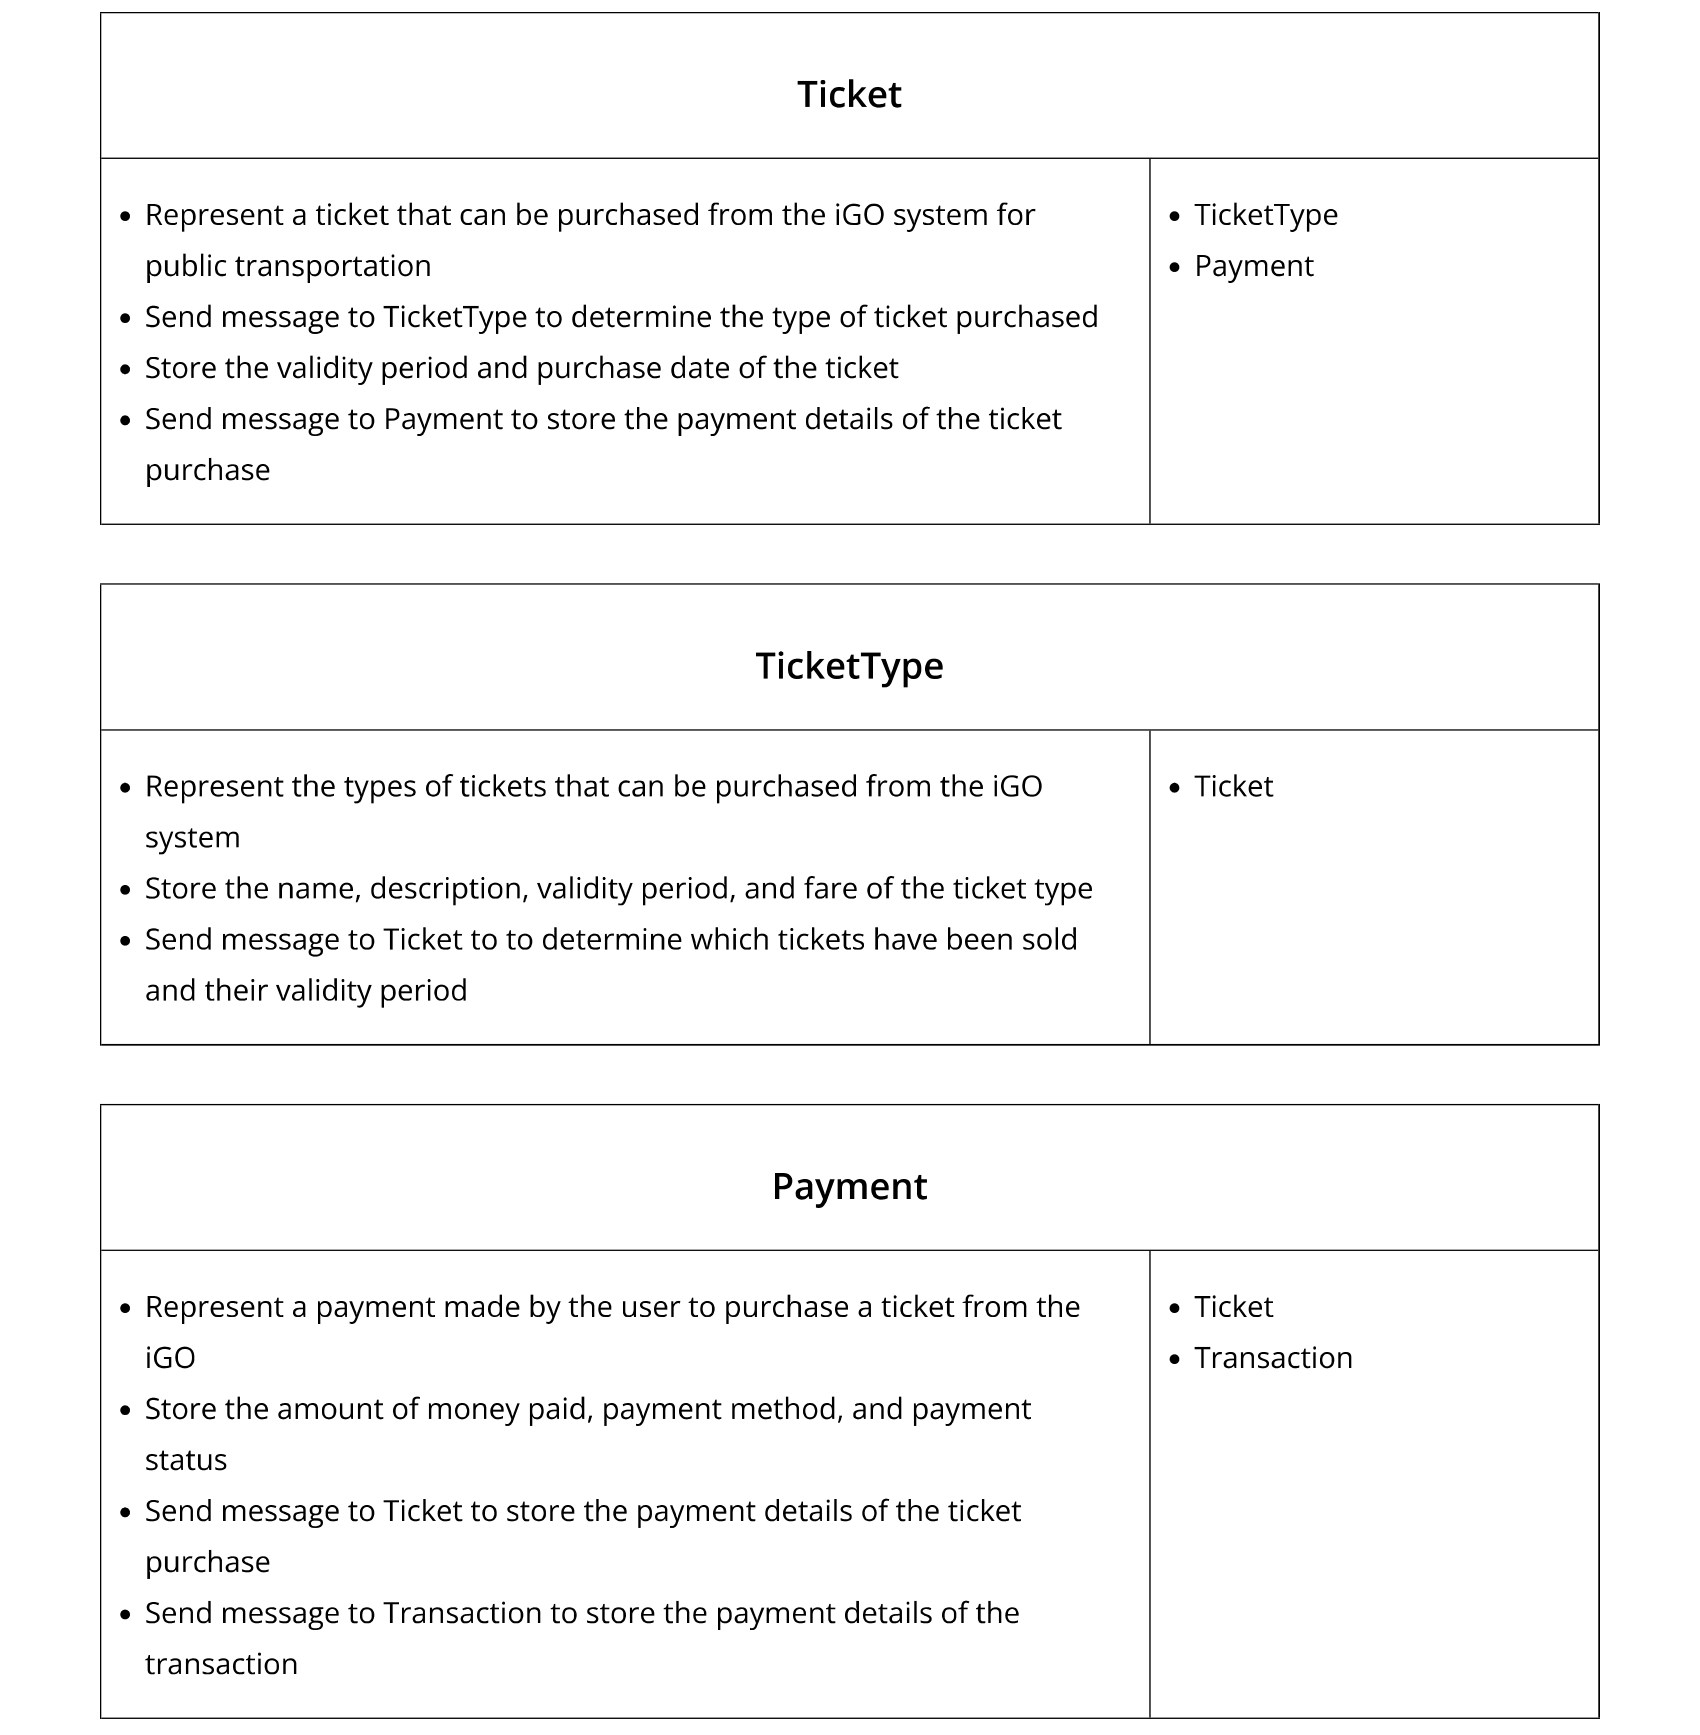
\includegraphics[width=\textwidth]{CRC-1.png} 
\end{figure}
\begin{figure}[t]
  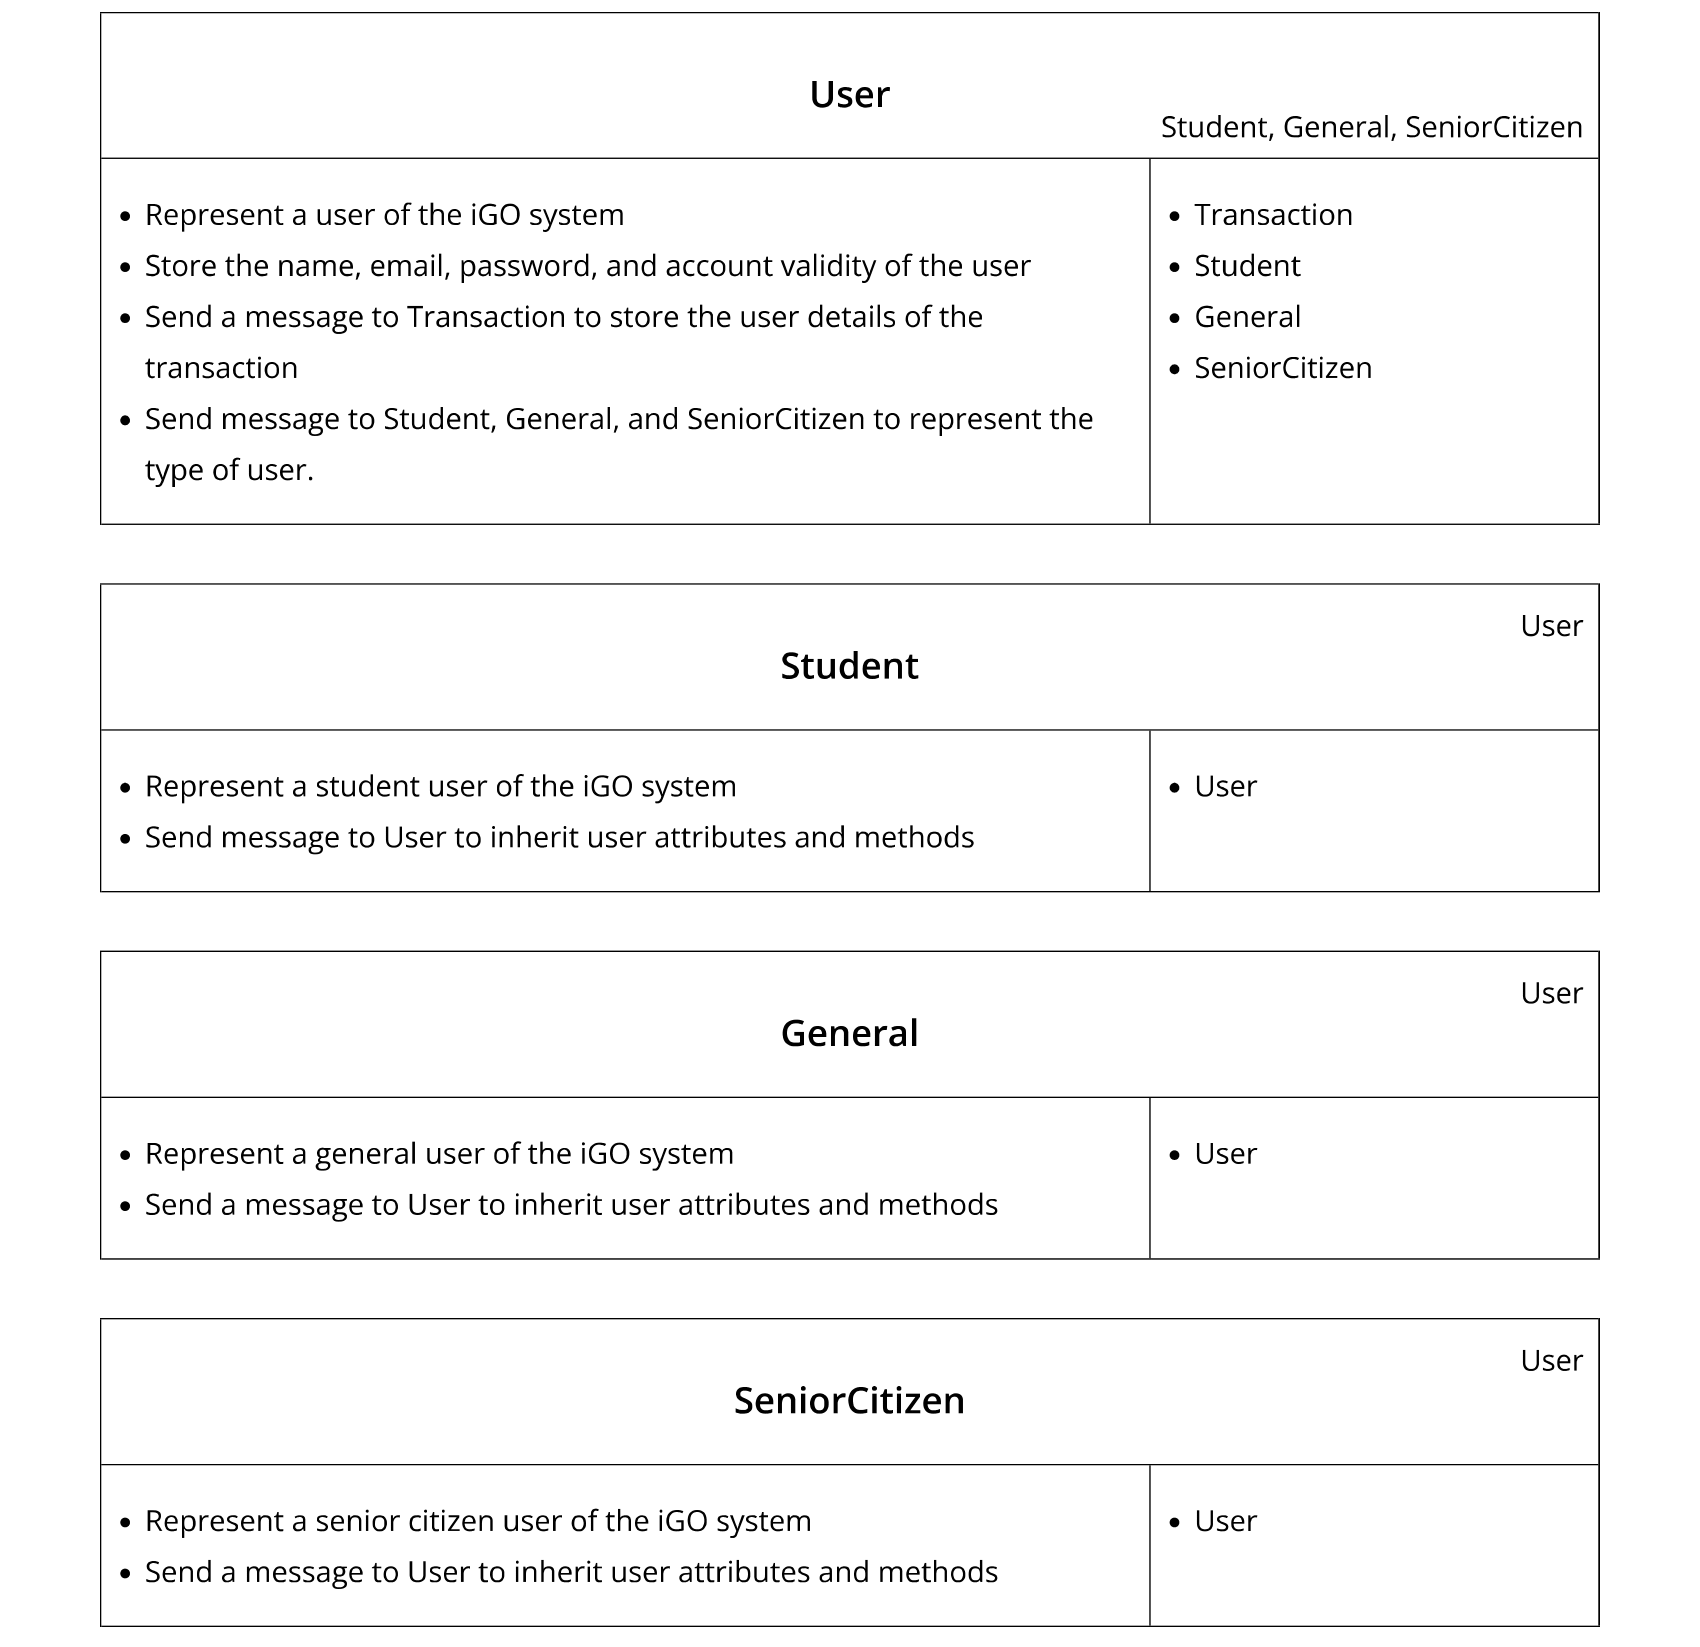
\includegraphics[width=\textwidth]{CRC-2.png} 
\end{figure}
\begin{figure}[h]
  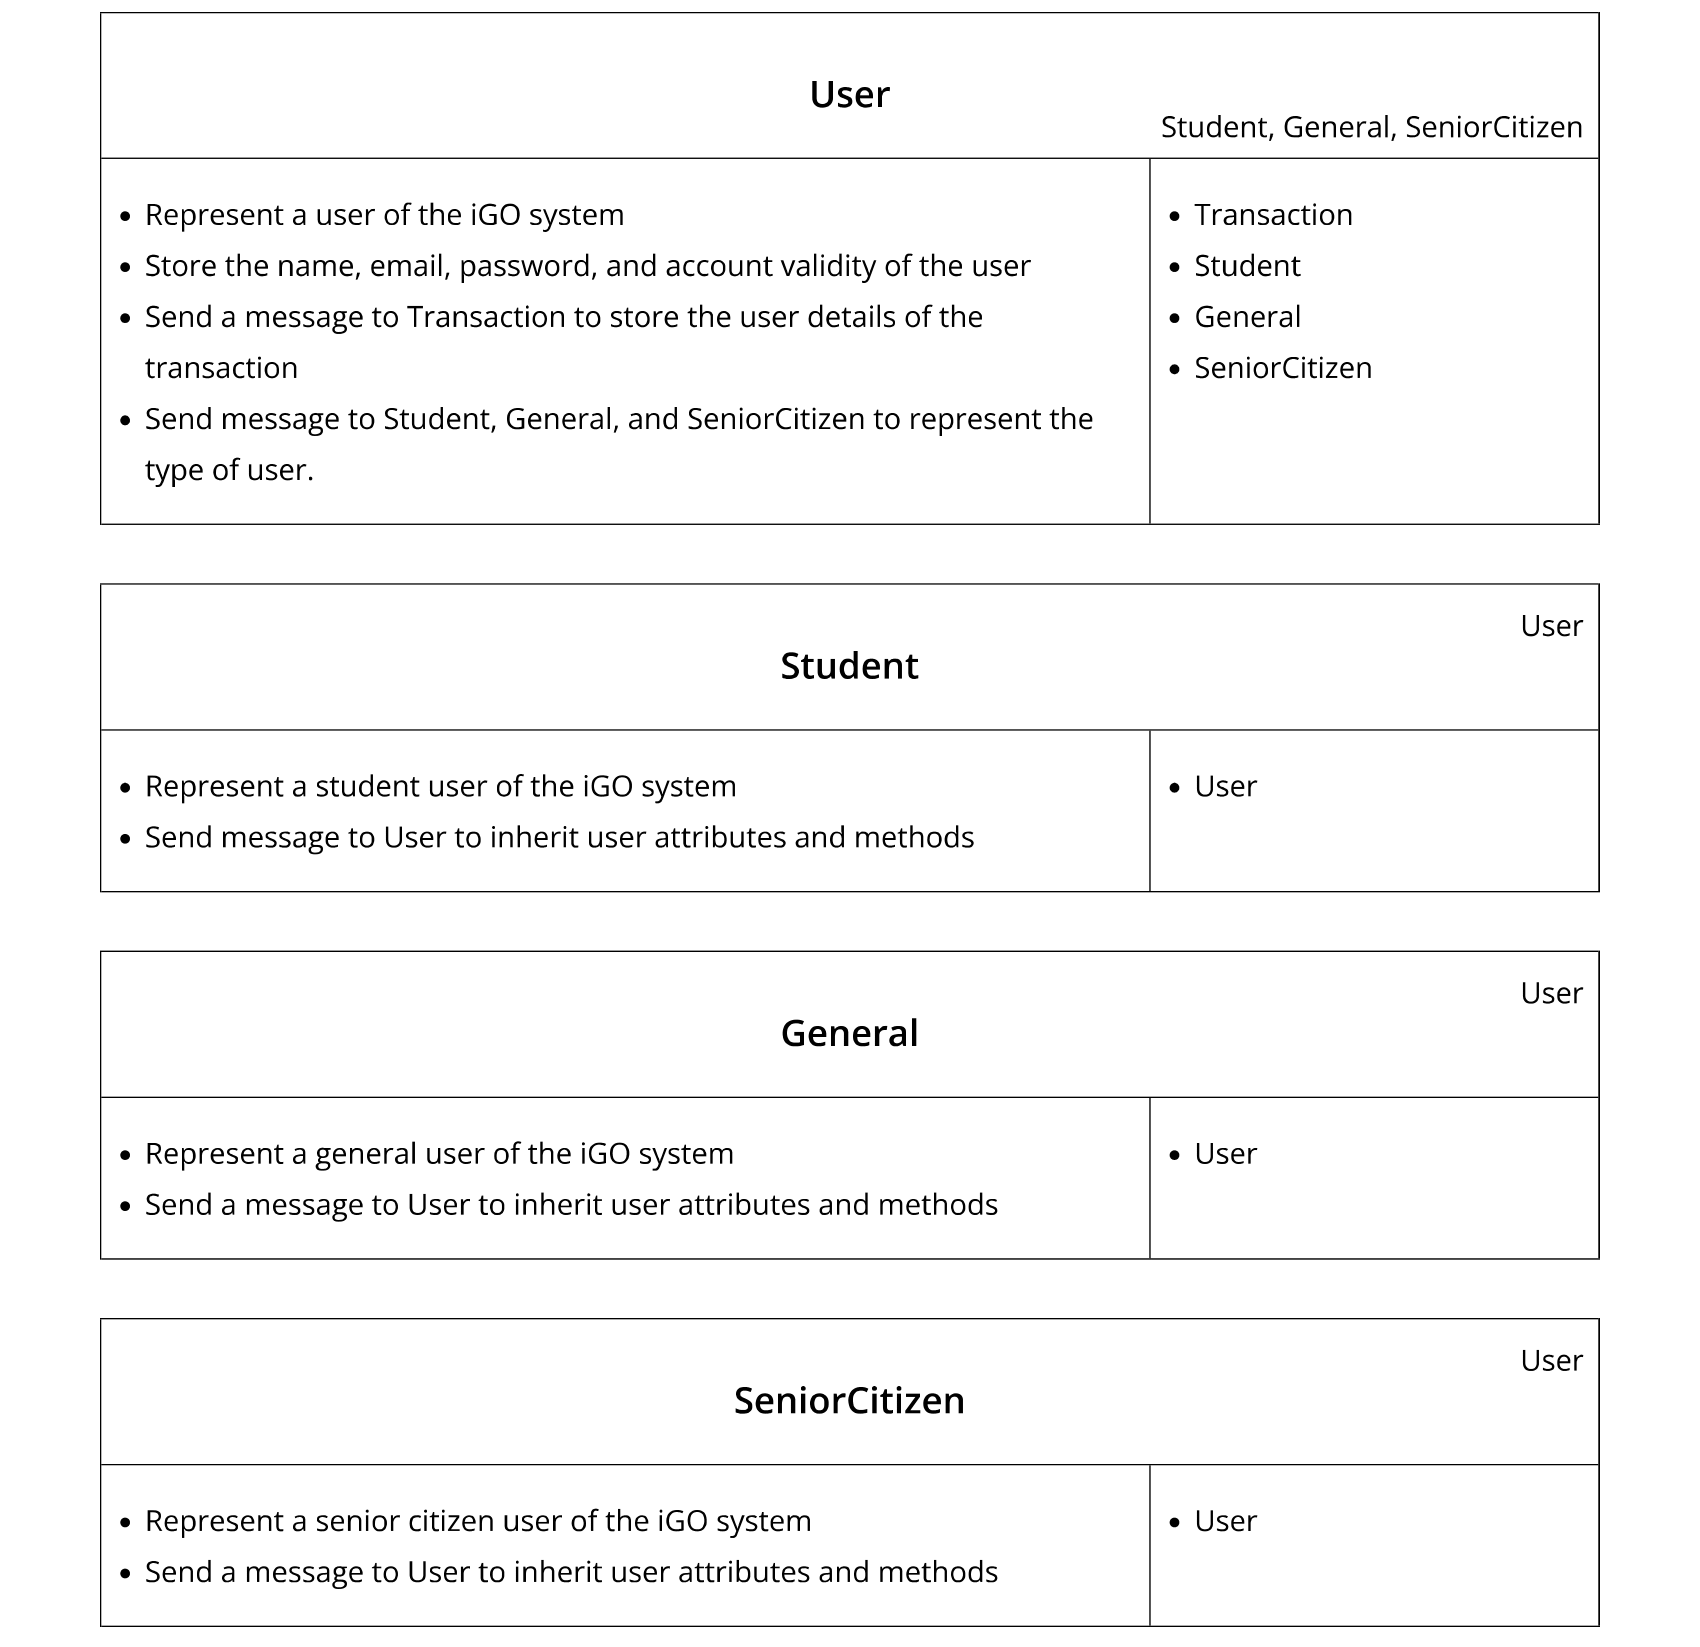
\includegraphics[width=\textwidth]{CRC-2.png}   
\end{figure}
\clearpage
\begin{figure}[h]
\renewcommand{\thefigure}{6.2.1}
    \centering
    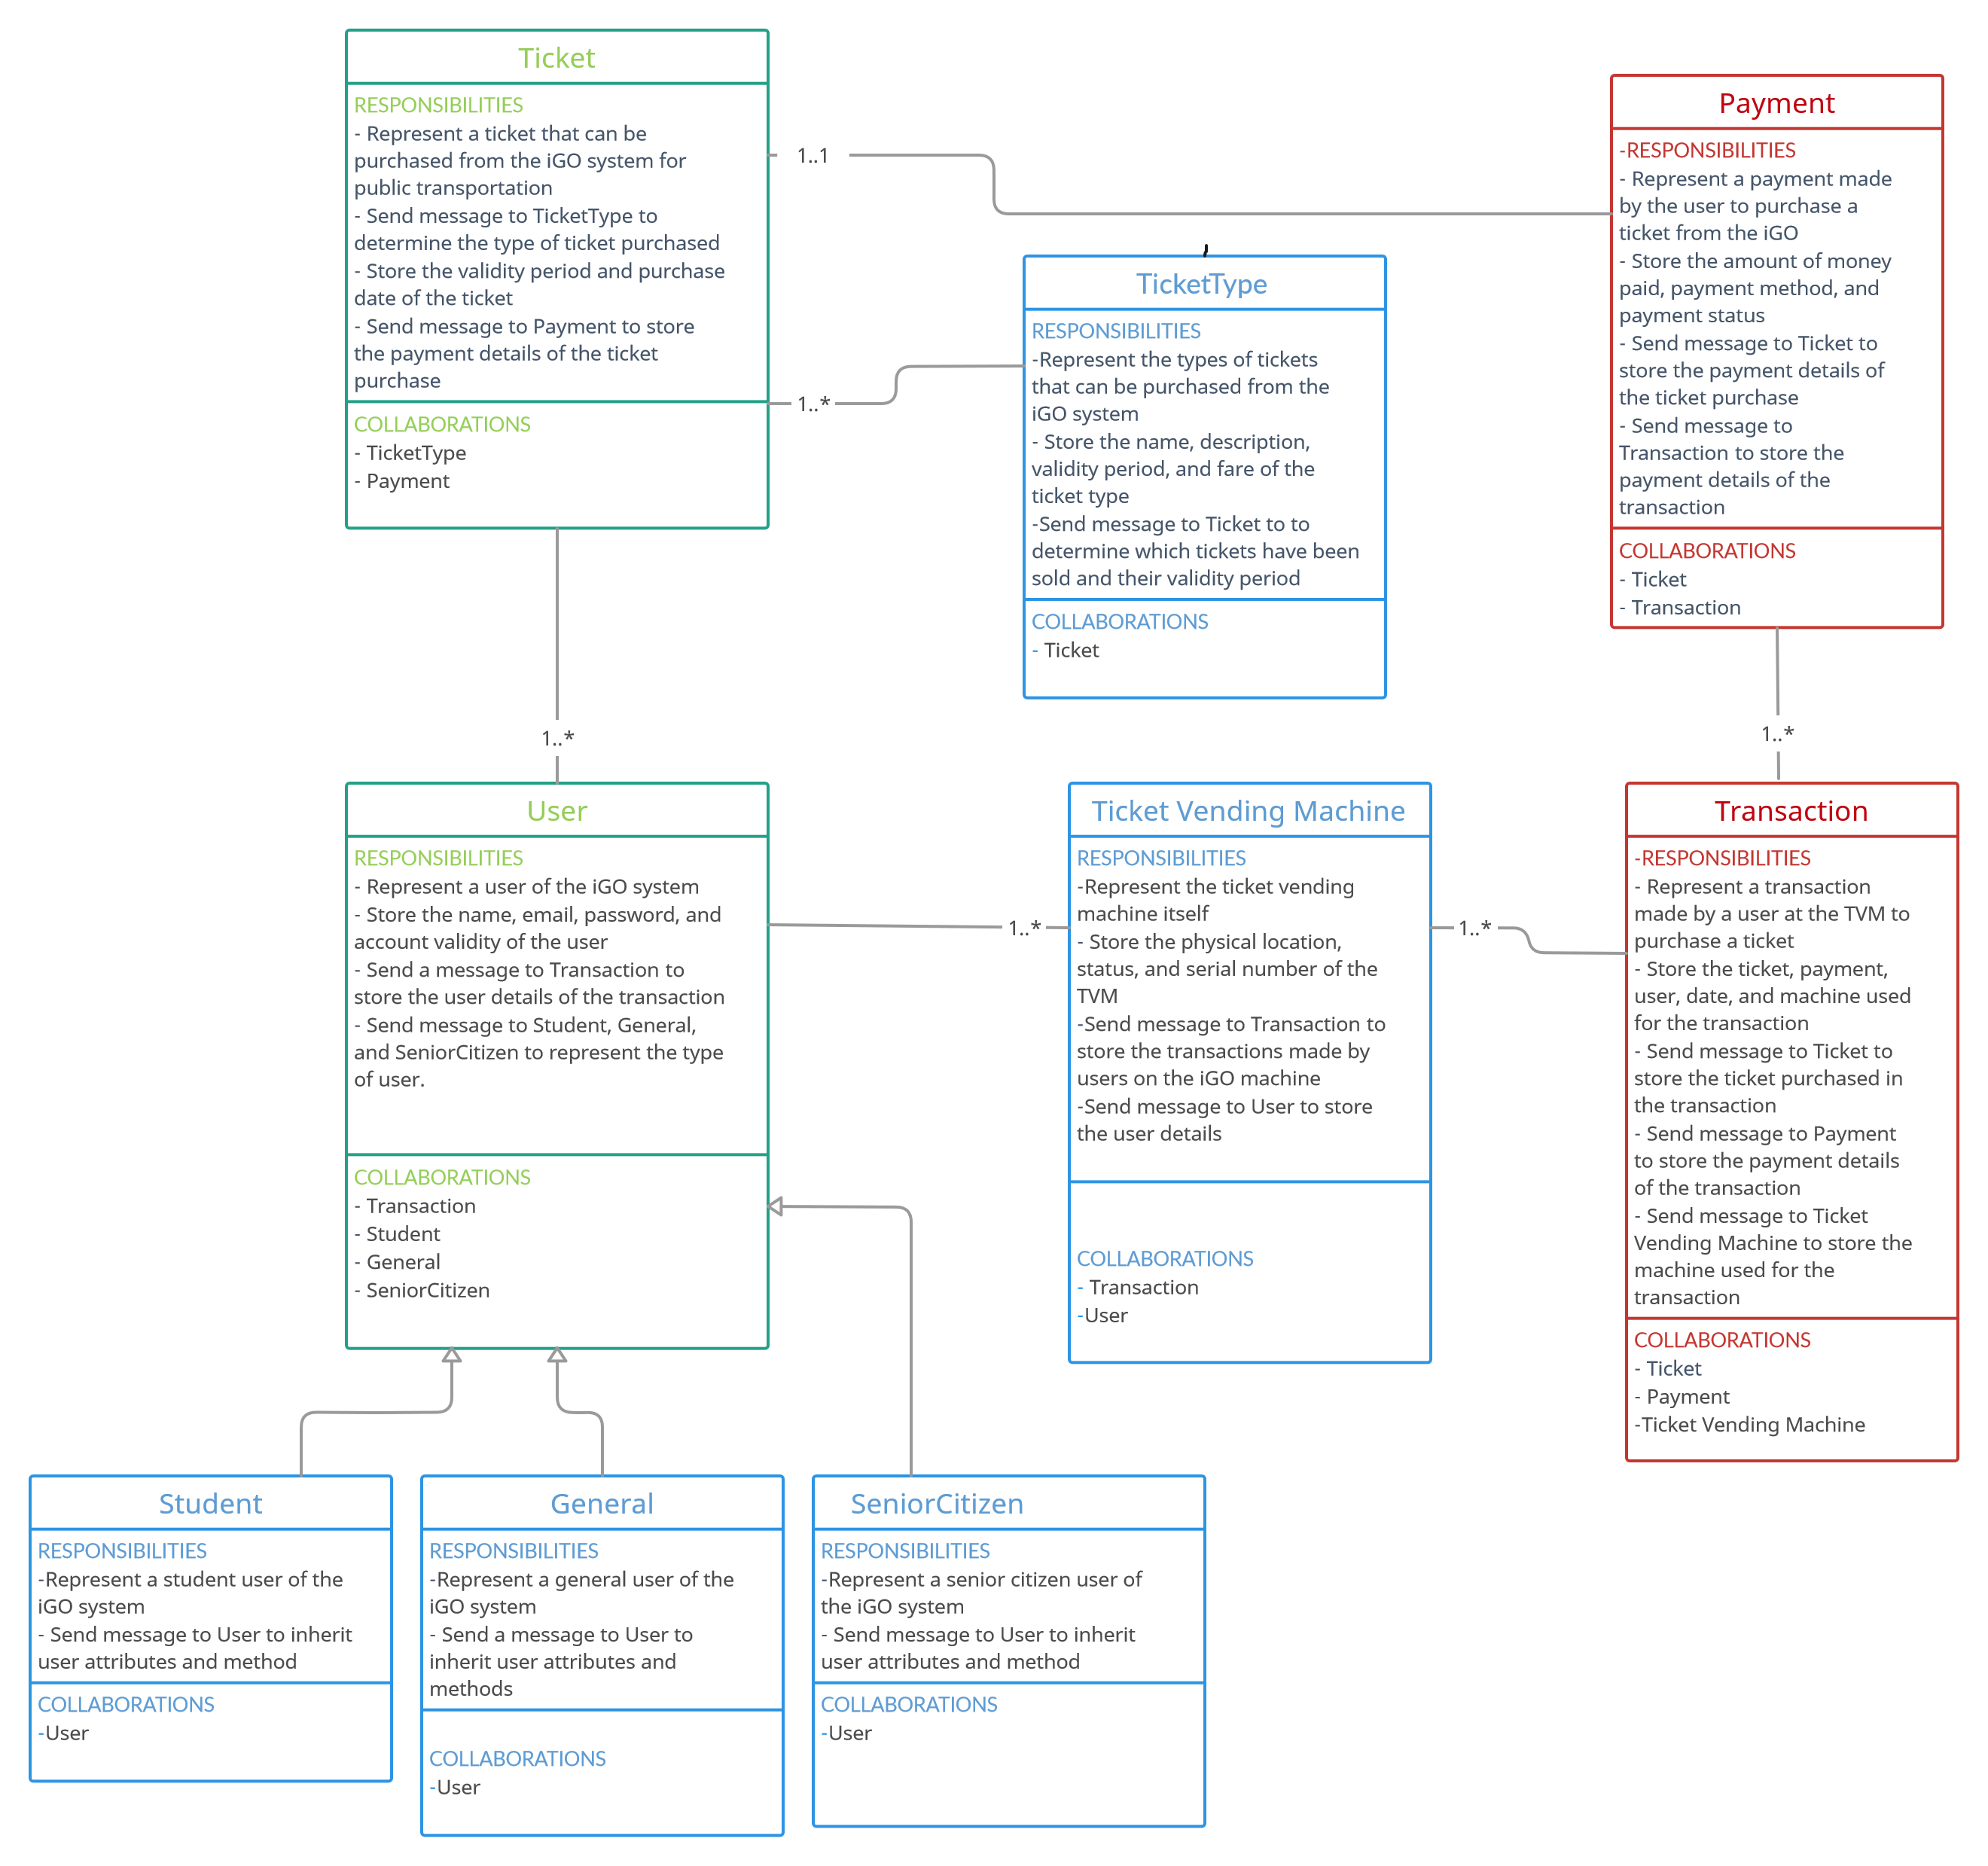
\includegraphics[width=\textwidth]{CRC card model.png}
    \caption{CRC Card Model}
     
\end{figure}


\chapter{Problem 7}
\renewcommand{\thesection}{7.\arabic{section}} % Redefine section numbering format
\section{UML Class Diagram}
\begin{figure}[h]
    \renewcommand{\thefigure}{7.1.1}
    \centering
    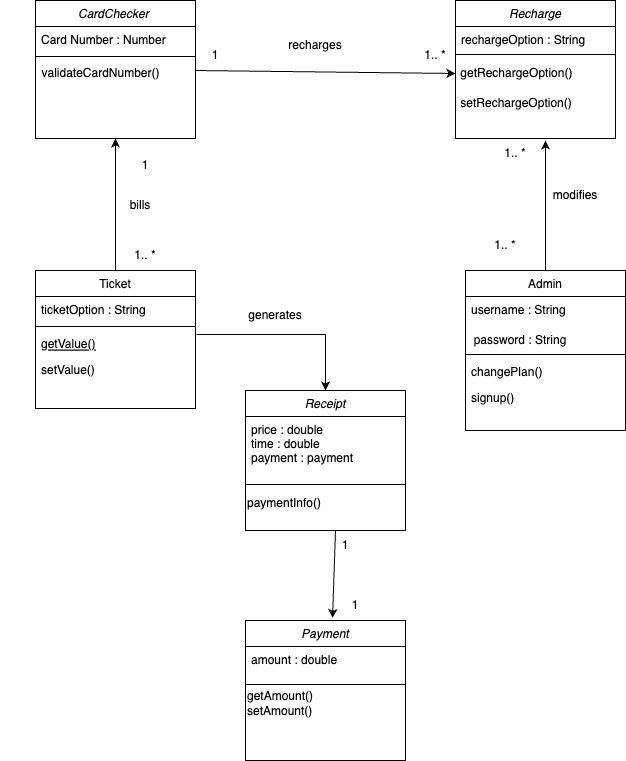
\includegraphics[scale=0.5]{UMLDiagram.jpg}
    \caption{UML Class Diagram}
\end{figure}
\clearpage  
A UML class diagram is a type of diagram used to depict the structure of a system by showing the classes of objects, their attributes, methods, and the relationships among them. Based on this requirement, I assume that iGo is a software system, and we need to create a class diagram to represent its structural design.\\

To begin with, we need to identify the classes in the iGo system. A class is a blueprint for creating objects, so we need to determine what objects we will need in iGo. \\
\begin{itemize}

  

   \item CardChecker: This class has a property called "card number" which is of type number. It also has a method called "validatecardnumber()" which presumably checks if the card number is valid.

    \item Recharge: This class has a property called "rechargeoption" which is of type string. It also has methods called "getrechargeoption()" and "setrechargeoption()" which are used to get and set the value of the "rechargeoption" property.

   \item Ticket: This class has a property called "ticketOption" which is of type string. It also has methods called "getvalue()" and "setvalue()" which are used to get and set the value of the "ticketOption" property.

   \item Admin: This class has two properties: "username" and "password", both of which are of type string. It also has methods called "changeplan()" and "signup()" which presumably allow the admin to change the plan and sign up new users.

   \item Receipt: This class has three properties: "price" and "time" both of which are of type double, and "payment" which is of type Payment (another class). It also has a method called "paymentinfo()" which is used to retrieve information about the payment.

   \item Payment: This class has one property called "amount" which is of type double. It also has methods called "getAmount()" and "setAmount()" which are used to get and set the value of the "amount" property.
\end{itemize}

\clearpage
\renewcommand{\thesection}{7.\arabic{section}} % Redefine section numbering format
\section{Sequence Diagram}
\subsection{Login}
The Login Sequence Diagram for iGo Ticket Vending Machine depicts the process of logging into the system. The diagram provides a clear overview of the steps involved in the login process, including the entry of user credentials, authentication, and the granting of system access. By following the flow of the diagram, users can gain a deeper understanding of the login process and the different stages involved. 
\begin{figure}[h]
    \renewcommand{\thefigure}{7.2.1}
    \centering
    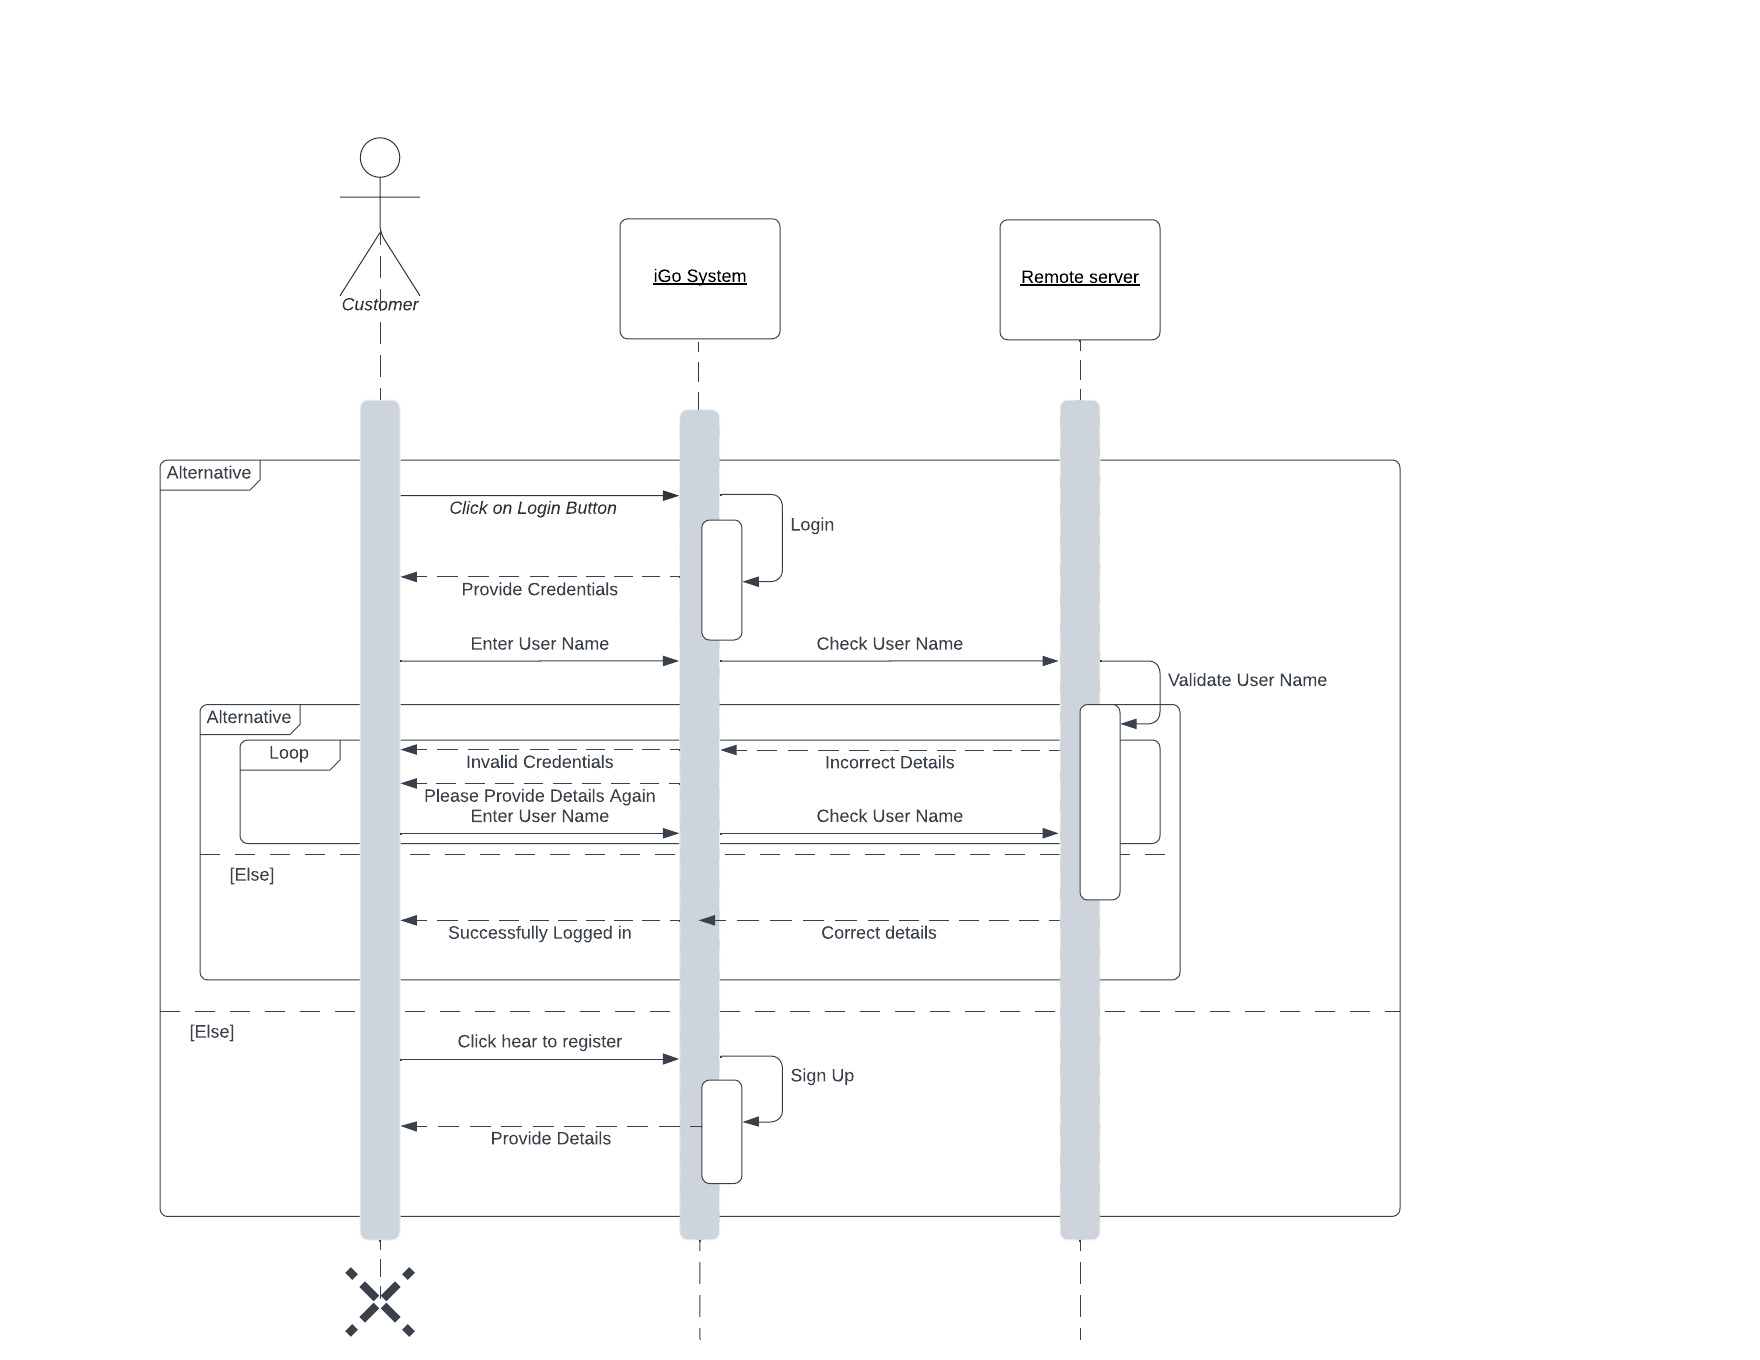
\includegraphics[scale=0.7]{Login.jpeg}
    \caption{Login Sequence Diagram}
\end{figure}
\clearpage
\subsection{Sign Up}
The Sign up Sequence Diagram for iGo System illustrates the process of registering a new user with the system. This diagram provides a step-by-step guide for users to easily understand how they can sign up for the iGo System and gain access to its features. The diagram outlines the various stages involved in the registration process, including the entry of personal information, validation of the information provided, and the creation of a user account. By following the flow of the diagram, users can easily navigate the registration process and become familiar with the various steps involved. Once registered, users can take full advantage of the iGo System's features and benefits. 
\begin{figure}[h]
    \renewcommand{\thefigure}{7.2.2}
    \hspace{-2cm}
    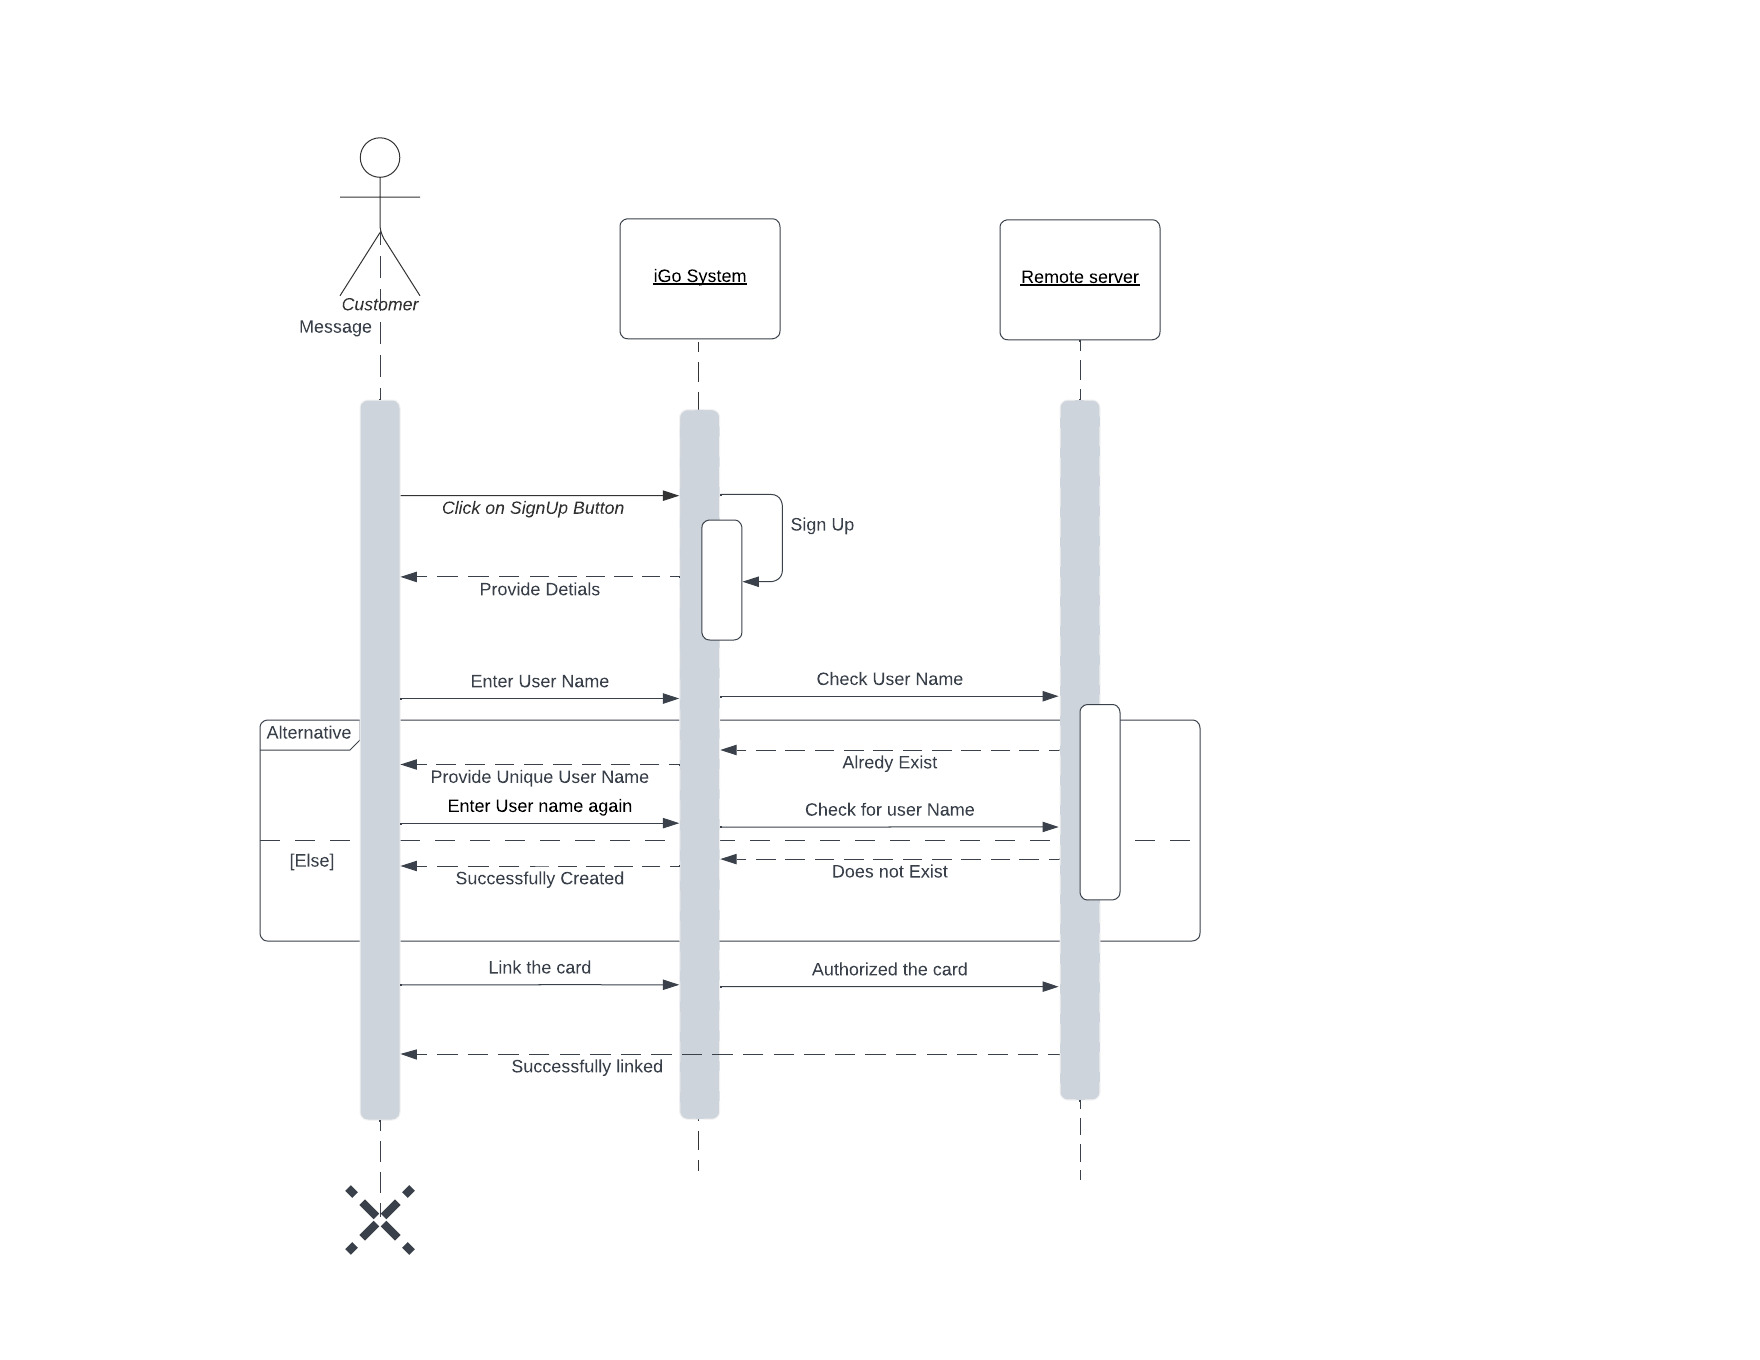
\includegraphics[scale=0.7,height=17cm]{SignUp.jpeg}
    \caption{Sign Up Sequence Diagram}
\end{figure}
\clearpage
\subsection{View Activity Details}
This Sequence Diagram outlines the processes involved in both logging into and signing up for the iGo System, as well as the ability for users to update their profile. To log in, users must have valid credentials, which they can obtain through the sign-up process. To sign up, new users must follow the steps outlined in the Sign up Sequence Diagram, which includes entering personal information and creating a user account. Once logged in, users can access their profile, which contains their personal information and other details. Users can also update their profile as needed, making changes to their information or preferences. By following the flow of the diagram, users can easily navigate these processes and take full advantage of the features and benefits of the iGo System. 
\begin{figure}[h]
    \renewcommand{\thefigure}{7.2.3}
    \hspace{1cm}
    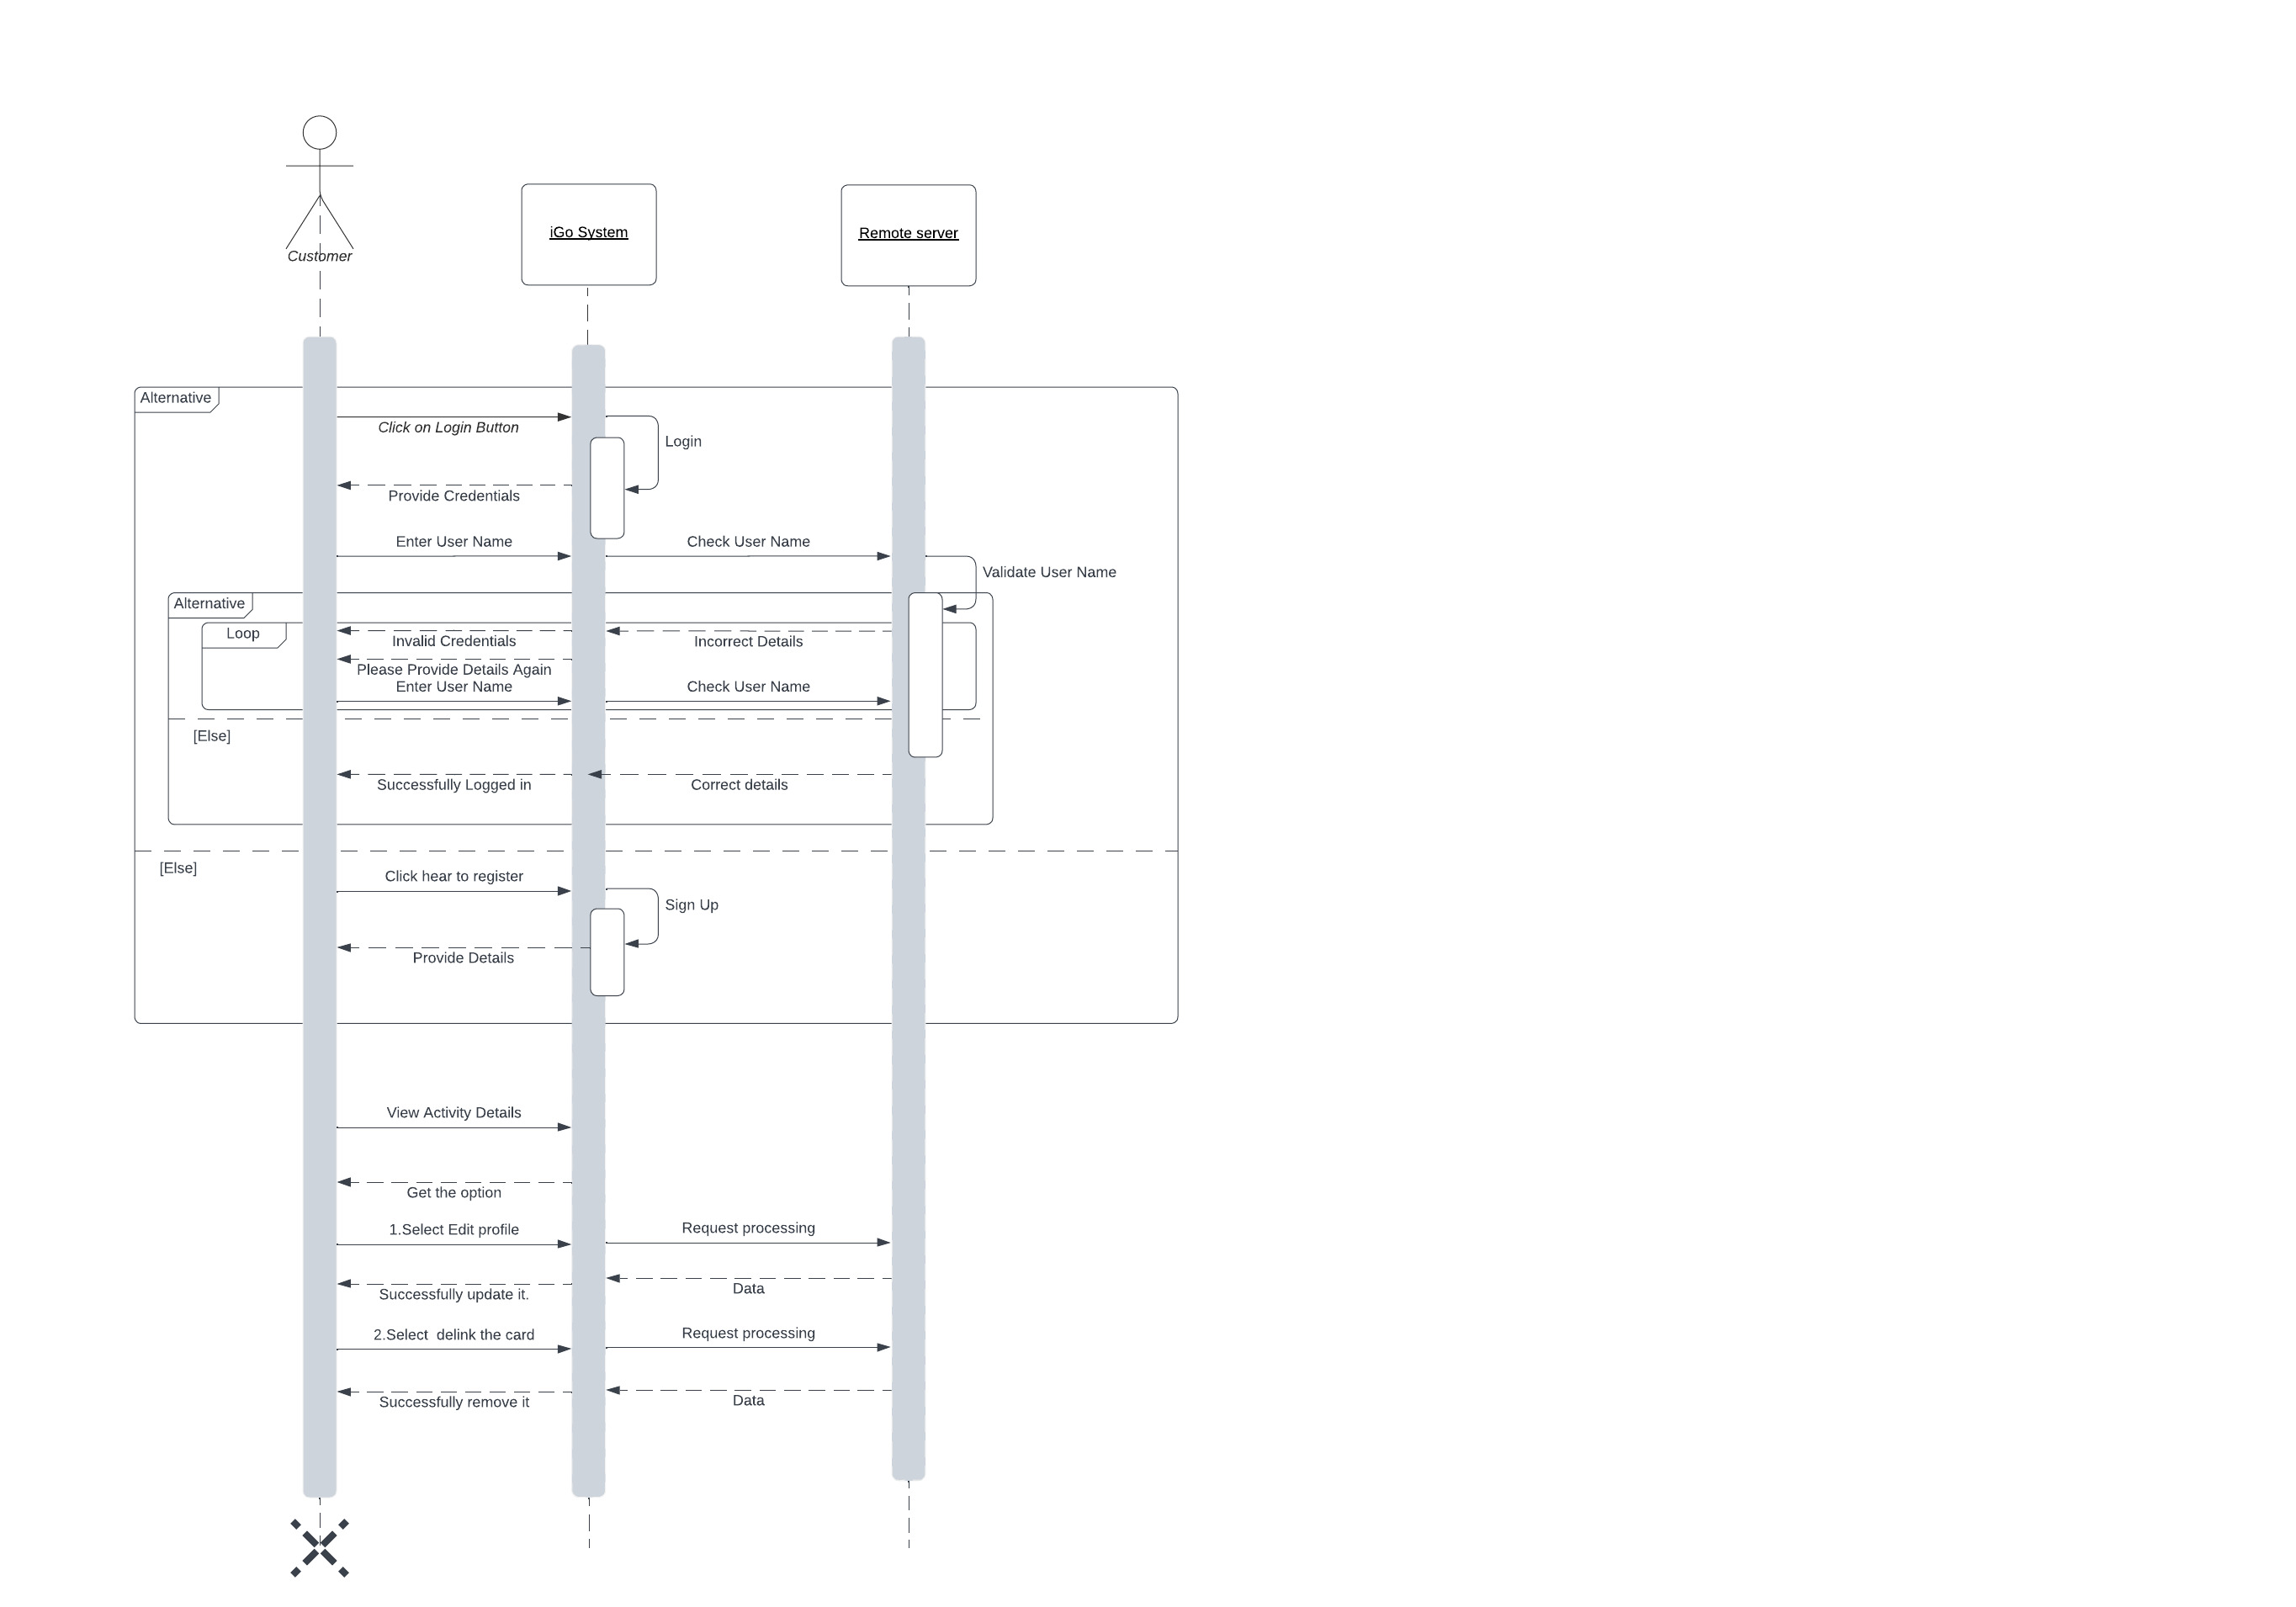
\includegraphics[scale=0.5,height=17cm]{ViewActivityDetails.jpeg}
    \caption{View Activity Details Sequence Diagram}
\end{figure}
\clearpage
\subsection{View Transaction History}
The View Transaction History feature of the iGo System provides users with an easy way to access details about their past transactions within the system. By selecting the View Transaction History option, users can see a list of their previous transactions, including details such as the transaction date, time, and amount. Users can also select individual transactions to view more detailed information about each one. Additionally, the View Transaction History feature offers the option to print transaction records, providing users with a hard copy of their transaction history if needed. This feature is a valuable tool for users who need to keep track of their transaction history for accounting or other purposes. 
\begin{figure}[h]
    \renewcommand{\thefigure}{7.2.4}
    \hspace{1cm}
    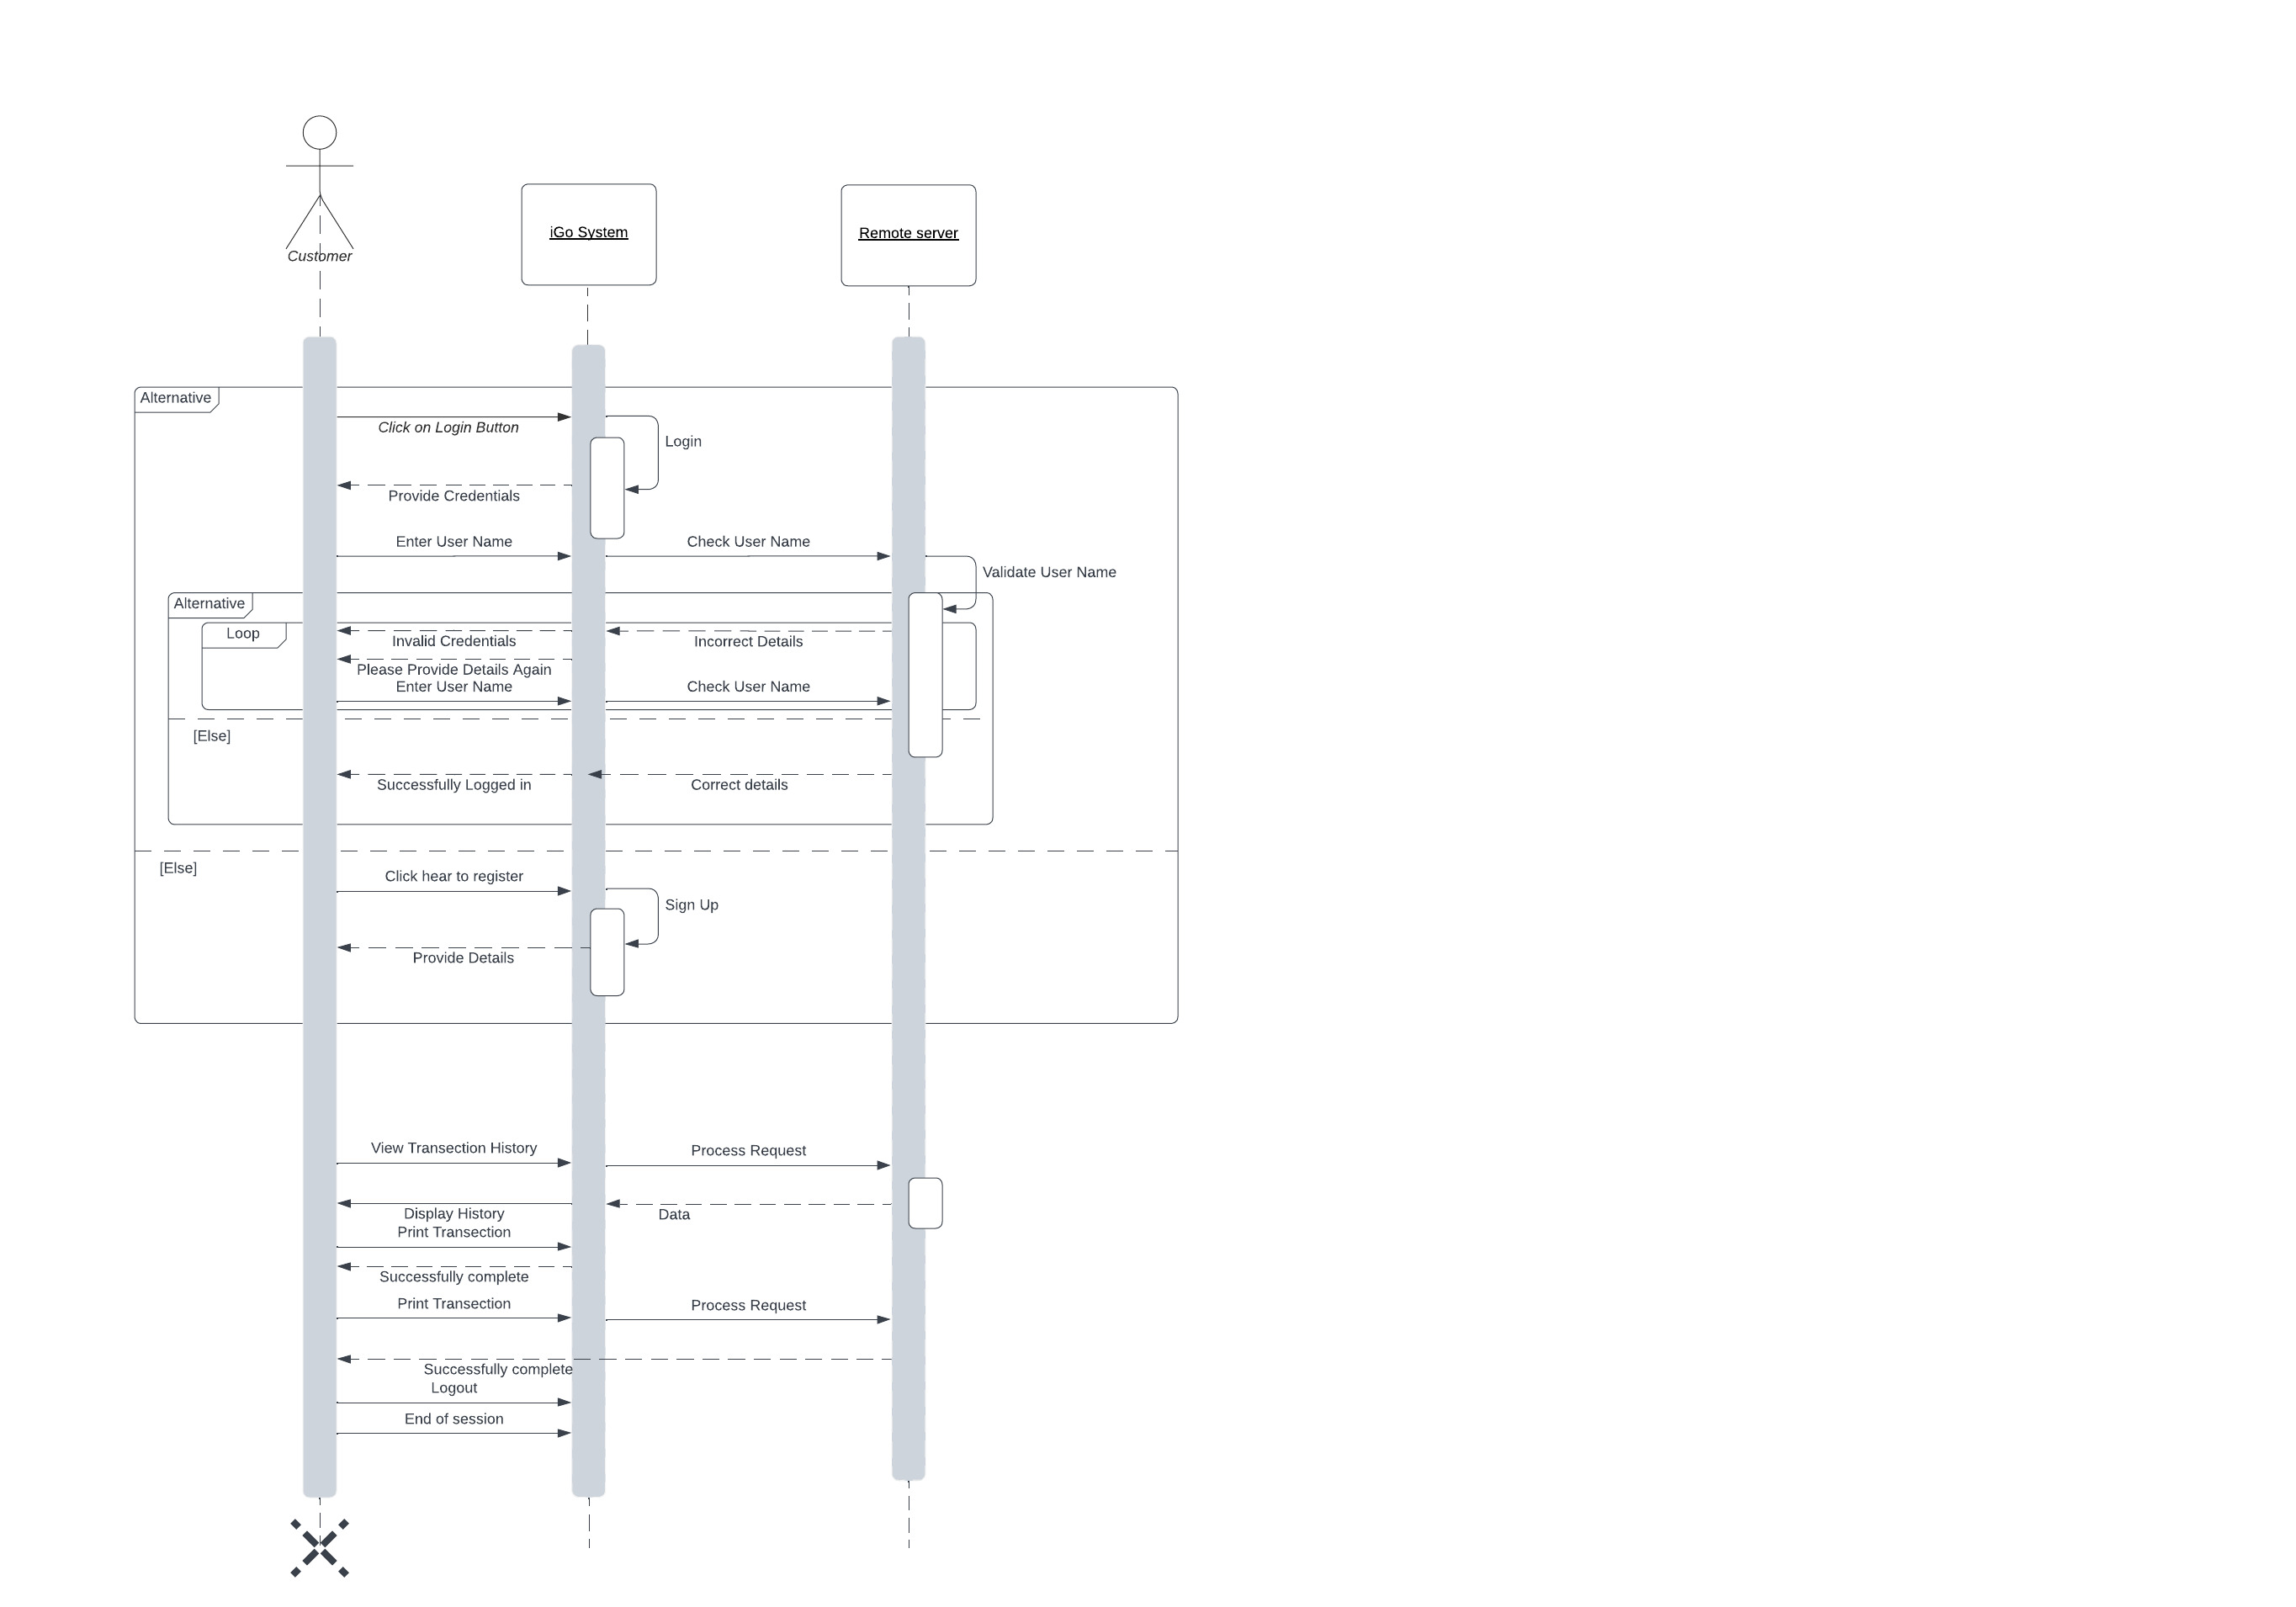
\includegraphics[scale=0.5,height=17cm]{ViewTransectionHistory.jpeg}
    \caption{View Transection History Sequence Diagram}
\end{figure}
\clearpage
\subsection{Purchase Ticket}
The ticket purchase process in the iGo System is represented in this Sequence Diagram. To purchase a ticket, users must first select the desired ticket type, and then proceed to the payment stage. The system provides users with various methods of payment, including credit card, debit card, and cash payment options. Once the payment has been processed and confirmed, the user receives a receipt for the transaction. This Sequence Diagram provides a clear and detailed overview of the ticket purchase process, from ticket selection to payment and receipt. 
\begin{figure}[h]
    \renewcommand{\thefigure}{7.2.5}
    \hspace{-4cm}
    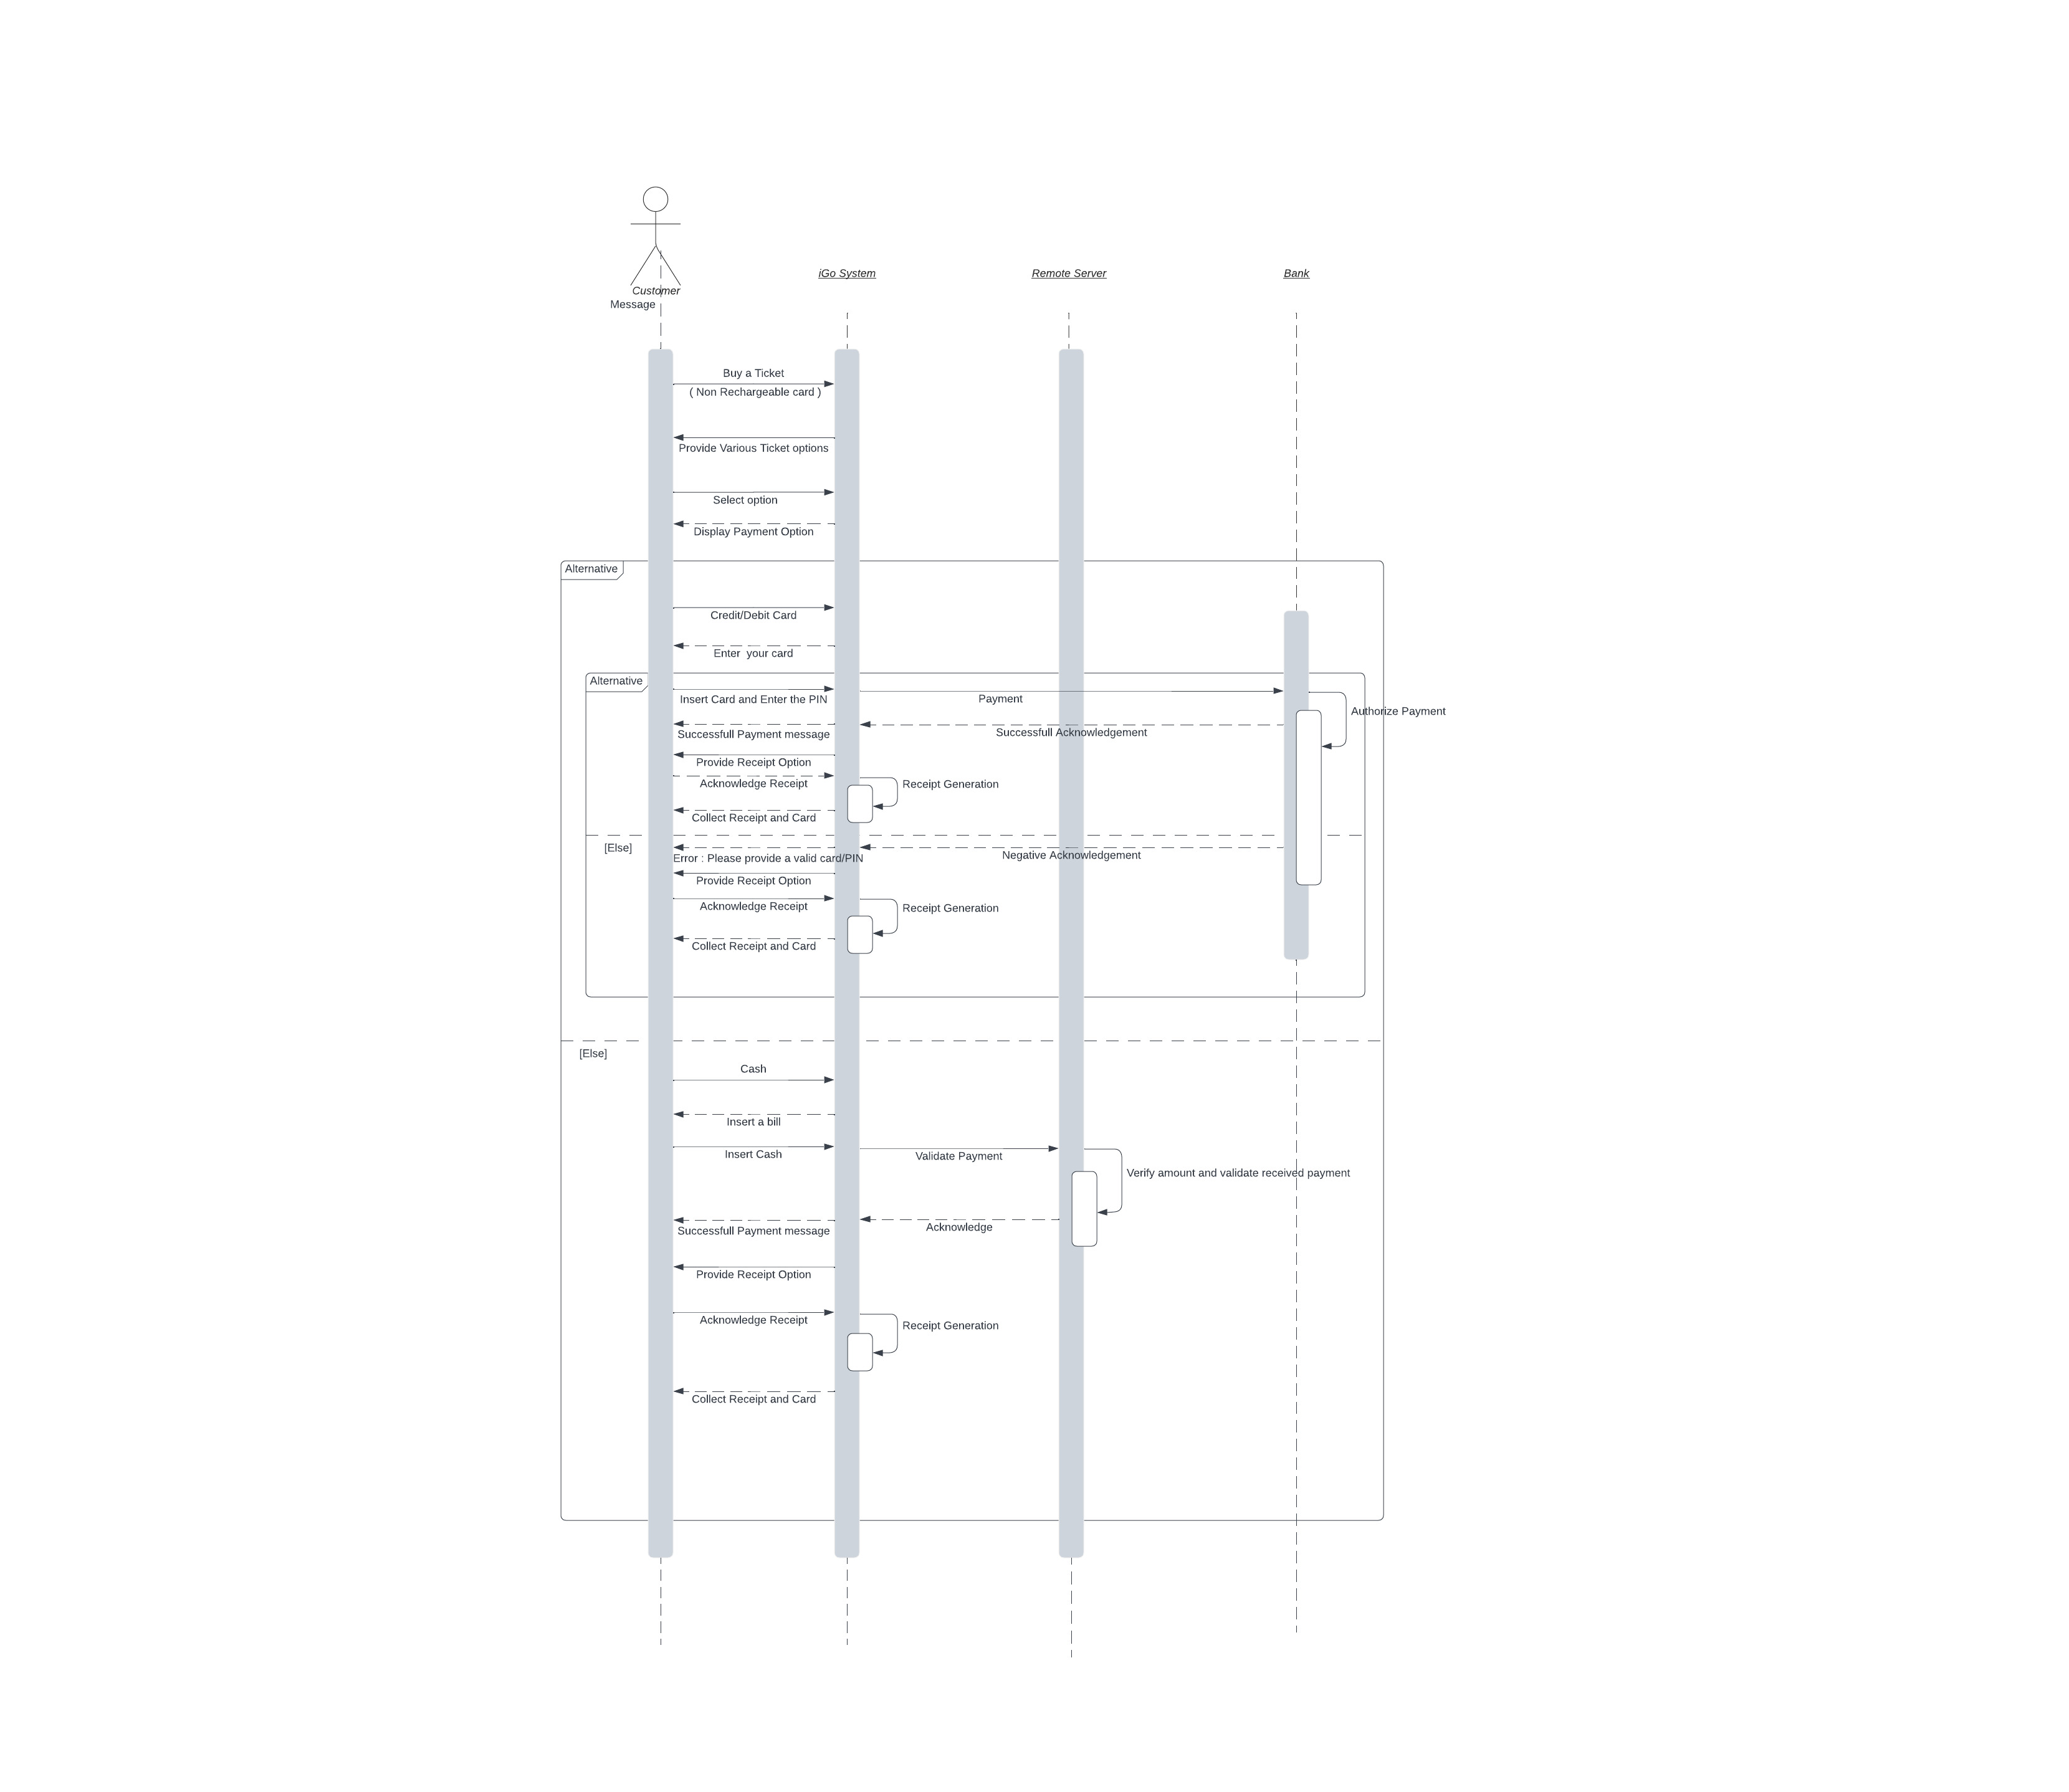
\includegraphics[width=25cm,height=17cm]{PurchaseTicket.jpeg}
    \caption{Purchase Ticket Sequence Diagram}
\end{figure}
\clearpage
\subsection{Make Payment}
This Sequence Diagram illustrates the payment process for the iGo System. To make a payment, users must first verify their identity through a secure authentication process. Once verified, users can select from a variety of payment options, including credit card, debit card, and cash. The system processes the payment and confirms the transaction, providing the user with a receipt for their records. The iGo System's user-friendly design ensures that making payments is a simple and straightforward process for all users.
\begin{figure}[h]
    \renewcommand{\thefigure}{7.2.6}
    \centering
    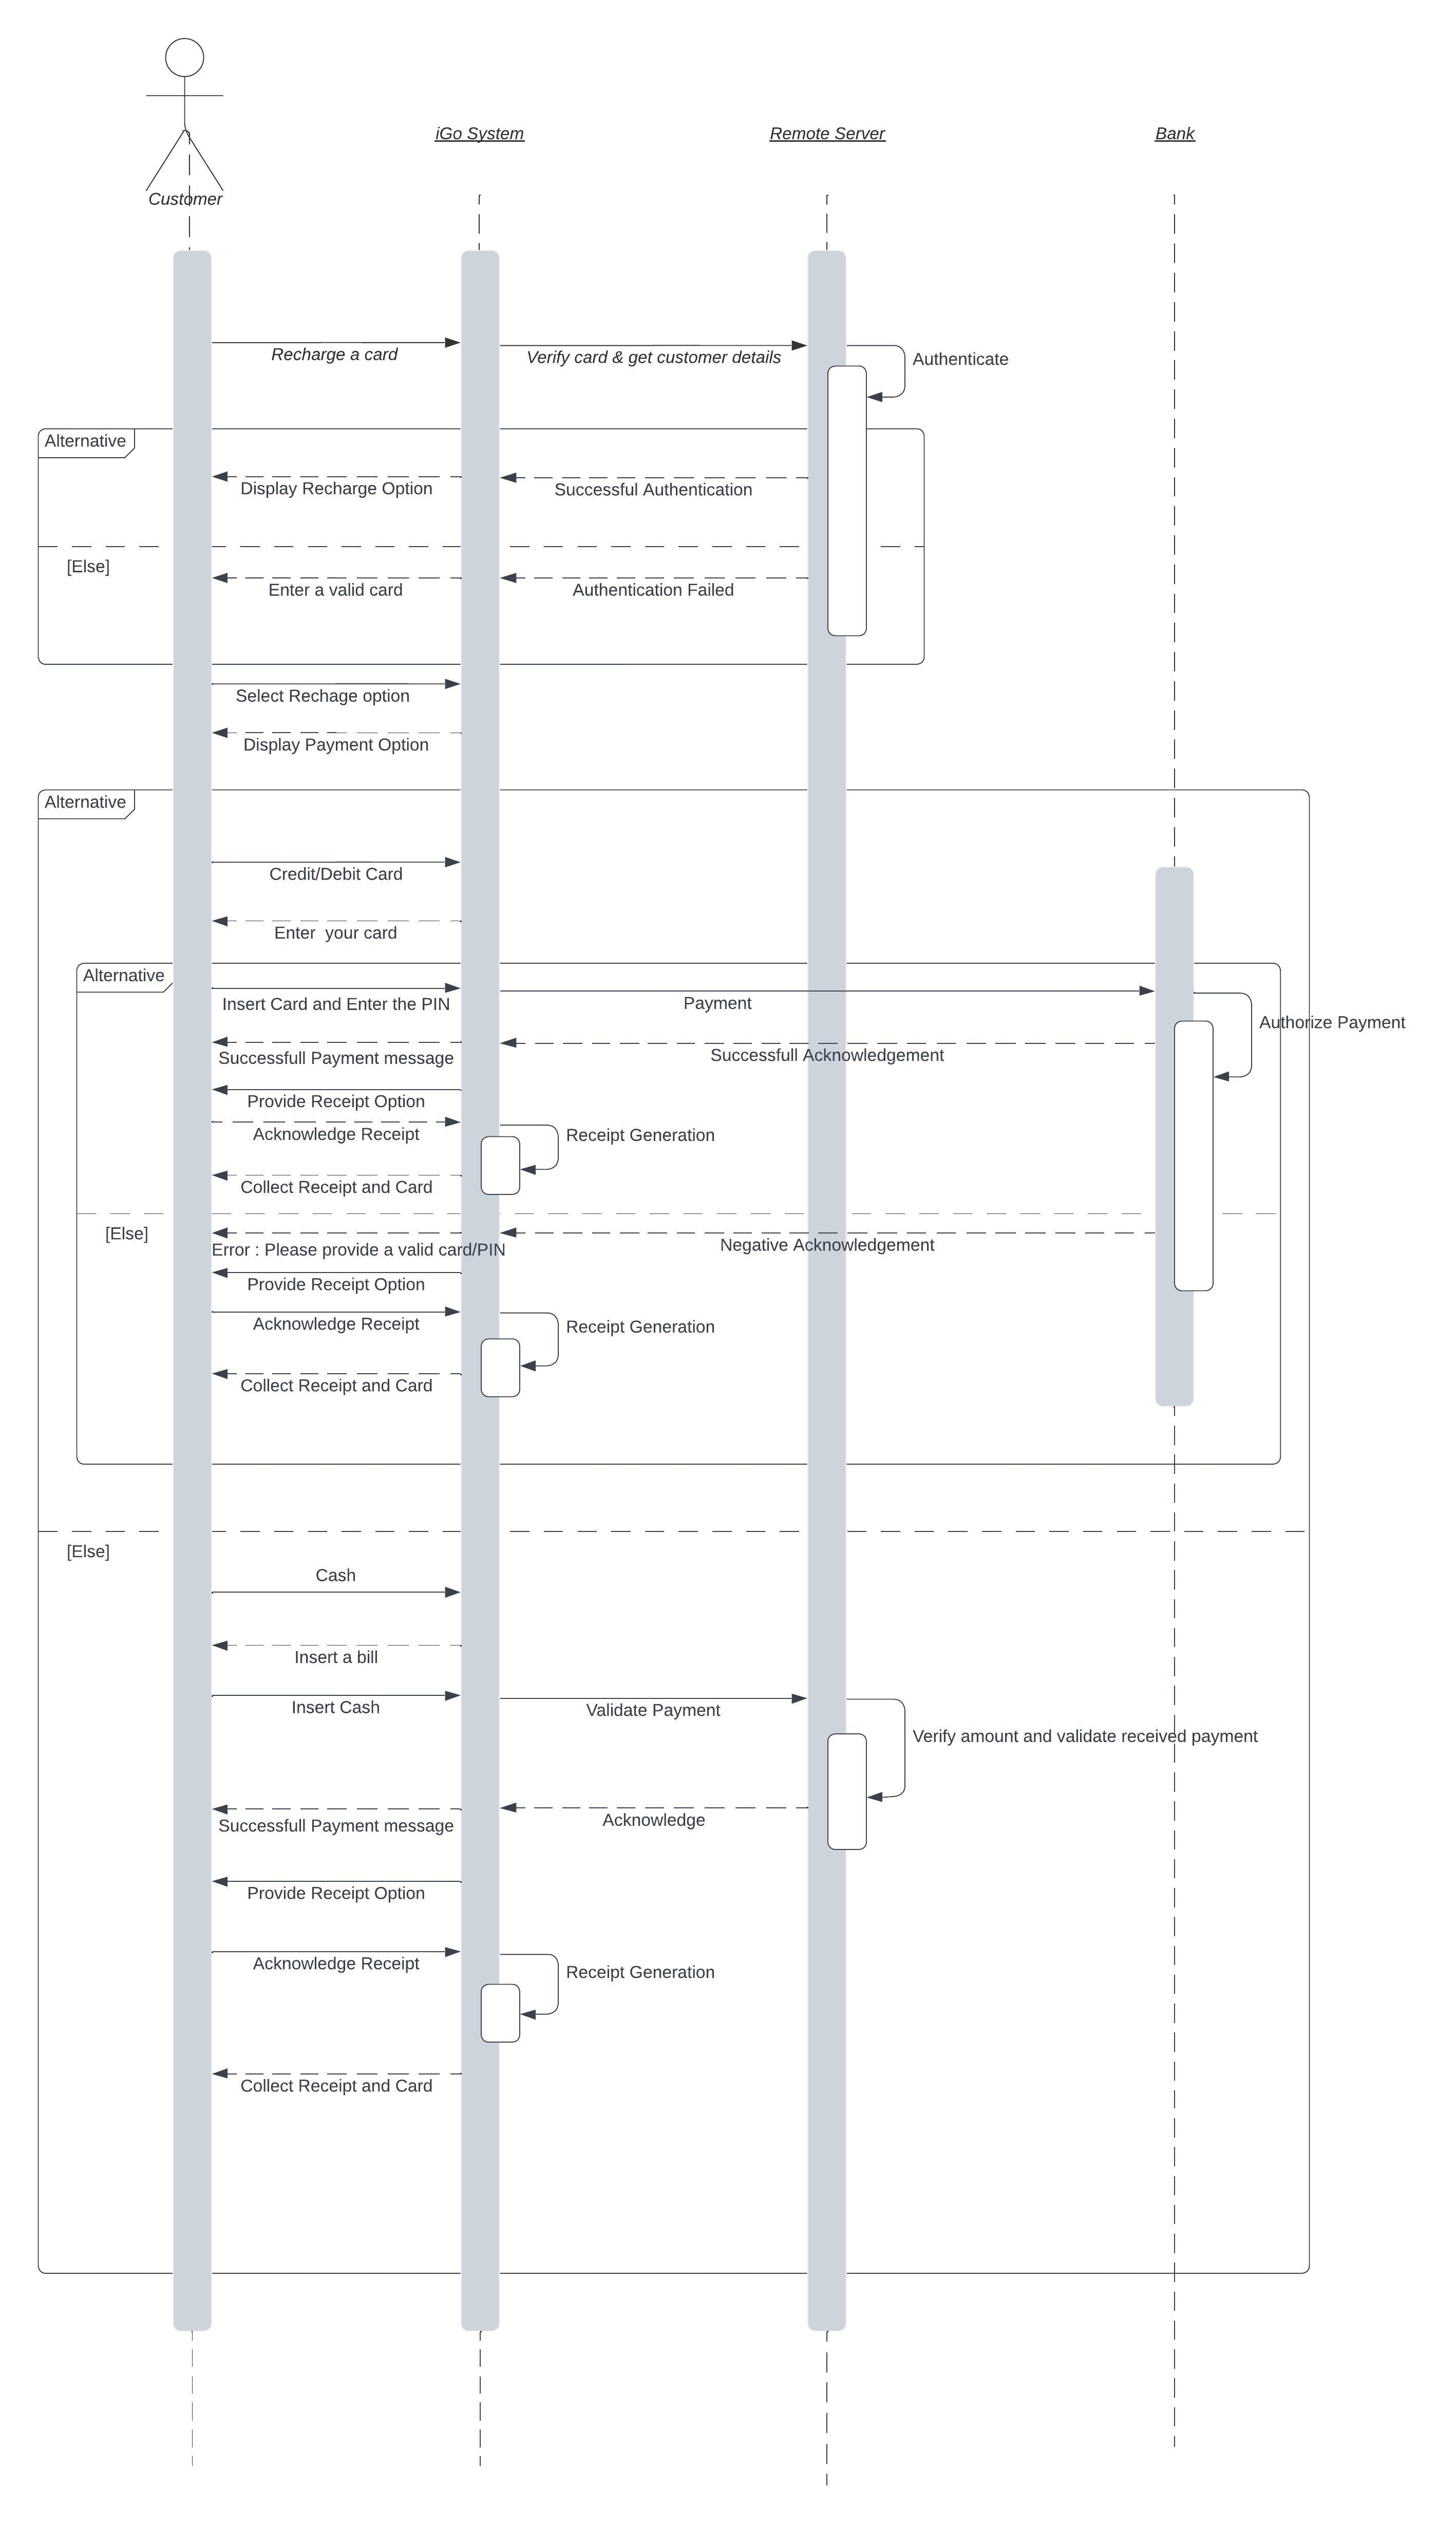
\includegraphics[width=10cm,height=17cm]{MakePayment.jpeg}
    \caption{Make Payment Sequence Diagram}
\end{figure}


\chapter{Problem 8}
Implementation of the code can be found at the following GitHub link:\\
\href{https://github.com/mahavir0/iGo---SOEN-6461-SDM}{https://github.com/mahavir0/iGo---SOEN-6461-SDM}
\\\\
We have used Java Swing GUI for the front end development. It provides a graphical user interface for users to purchase a new ticket, recharge a card, or access the admin panel.\\
There are several methods to create different screens for the TVM application. The mainPage method creates the main screen with buttons to purchase a new ticket, recharge a card, or access the admin panel. The rechargeCard method creates a screen with options for card recharge. The buyTicket method creates a screen with options for buying a new ticket. The adminPanel method creates a screen with options for the admin user to manage ticket and recharge plans. The paymentMethod method creates a screen with payment options for the user to complete their purchase.

\chapter{Problem 9}
\renewcommand{\thesection}{9.\arabic{section}} % Redefine section numbering format
\setcounter{section}{0} % Set section counter to start from 0
\section{Test Cases}
\subsection{Purchase New Ticket}
To purchase a new ticket, the user must navigate to the homepage and select the "Purchase a New Ticket" option. From there, the user will be presented with various ticket types to choose from. Next, the user will be prompted to select a method of payment, which includes the option to pay by card or cash. If the user selects the card payment option, they must input valid card details to complete the transaction. Conversely, if the user opts for cash payment, they will need to enter the exact amount of cash and collect any change due. Users will then be given the option to receive the receipt via email or print it at the iGO machine. Once all necessary requirements have been fulfilled, the iGO machine will display a "Thank You" message.\\
\begin{figure}[ht]
\centering
   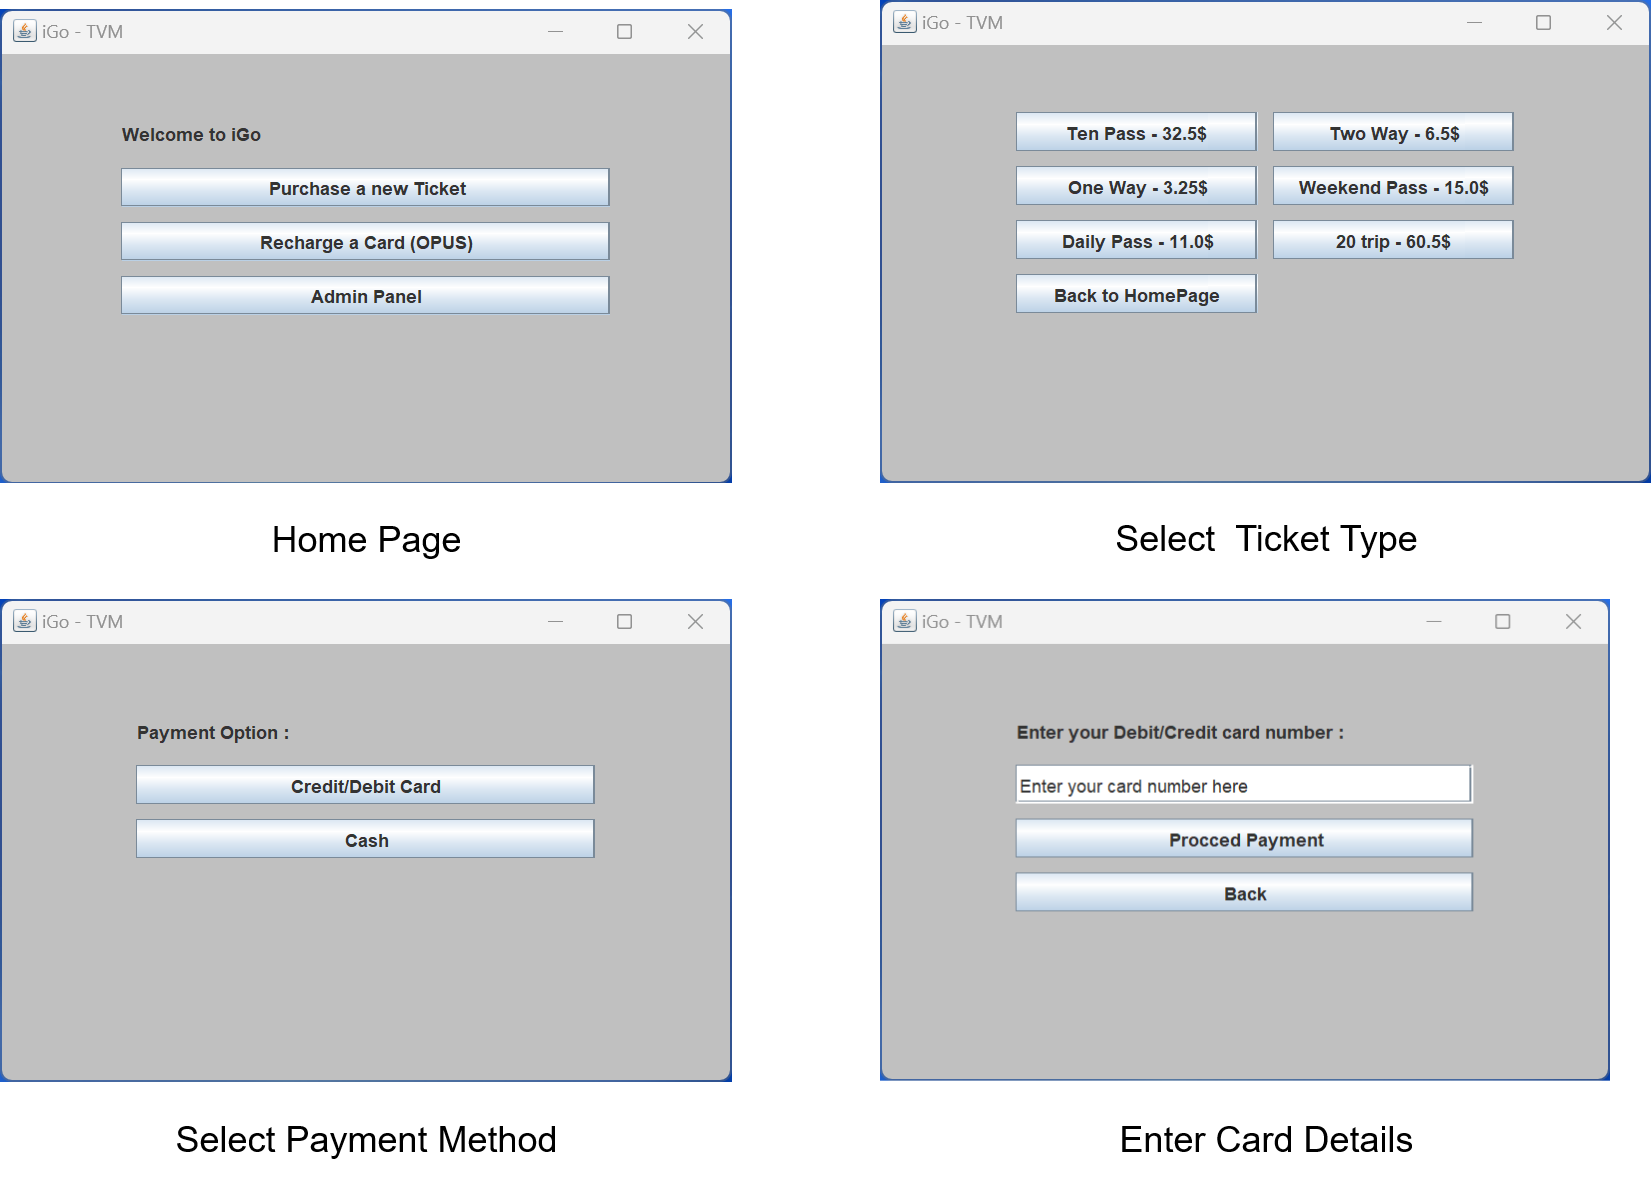
\includegraphics[width=14cm]{1.1.png} 
\end{figure}
\begin{figure}[ht]
\centering
    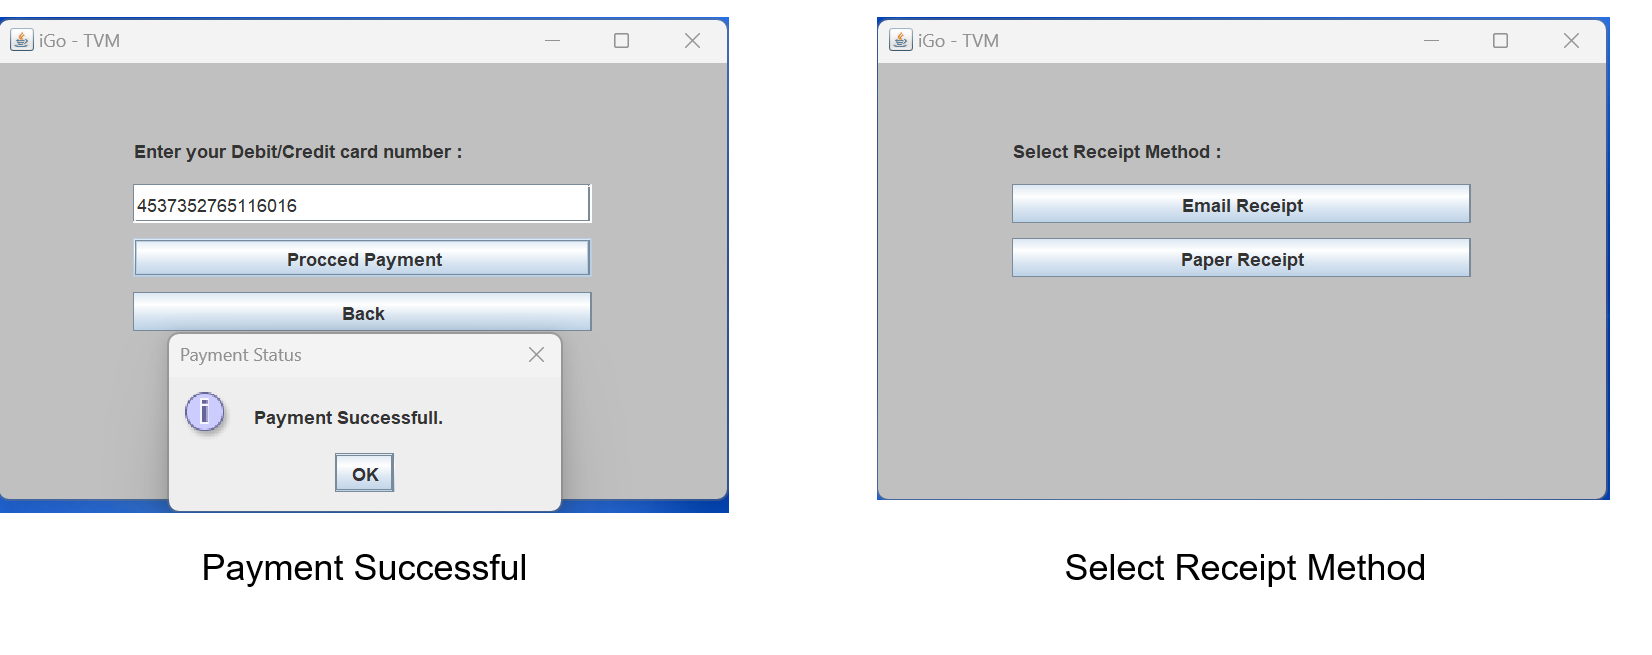
\includegraphics[width=14cm]{1.2.png} 
   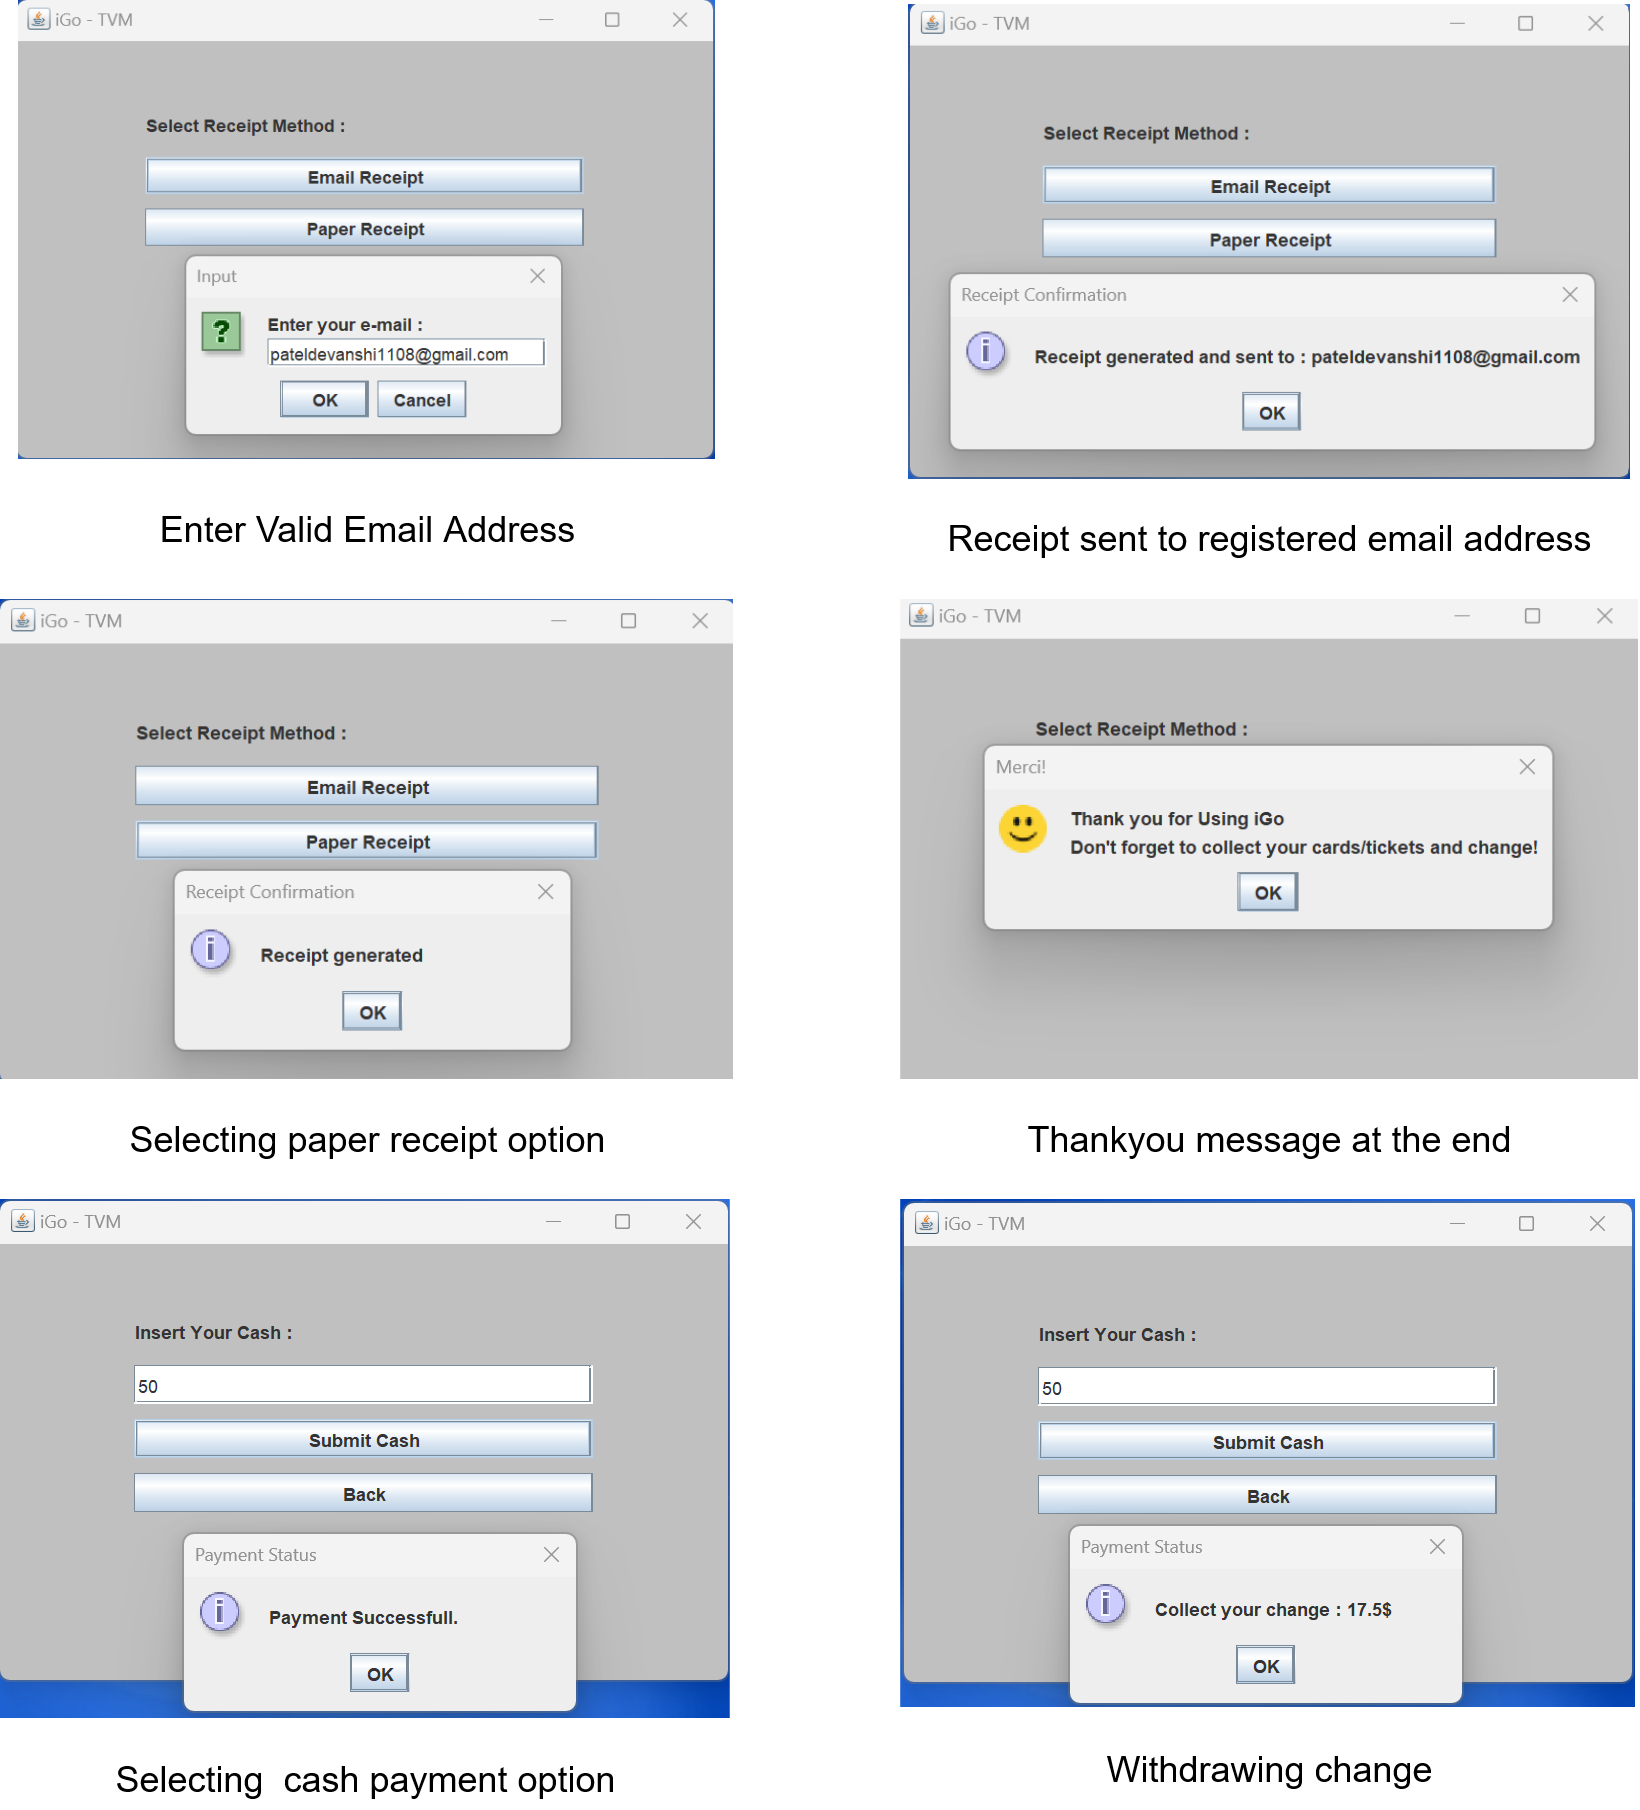
\includegraphics[width=14cm]{2.png} 
\end{figure}
\clearpage 
\subsection{Recharge Opus Card}
To recharge an Opus card, the user must first access the homepage and select the "Recharge a Card (Opus)" option. From there, the user will be presented with a variety of recharge options to choose from. Next, the user will need to select a payment method, which includes the option to pay via card or cash. If the user chooses to pay via card, they will need to provide valid card information to complete the transaction. Alternatively, if the user opts for cash payment, they will be required to enter the exact amount and collect any change due. Once all necessary requirements are met, a message confirming a successful recharge will be displayed.\\
\begin{figure}[h]
\centering
   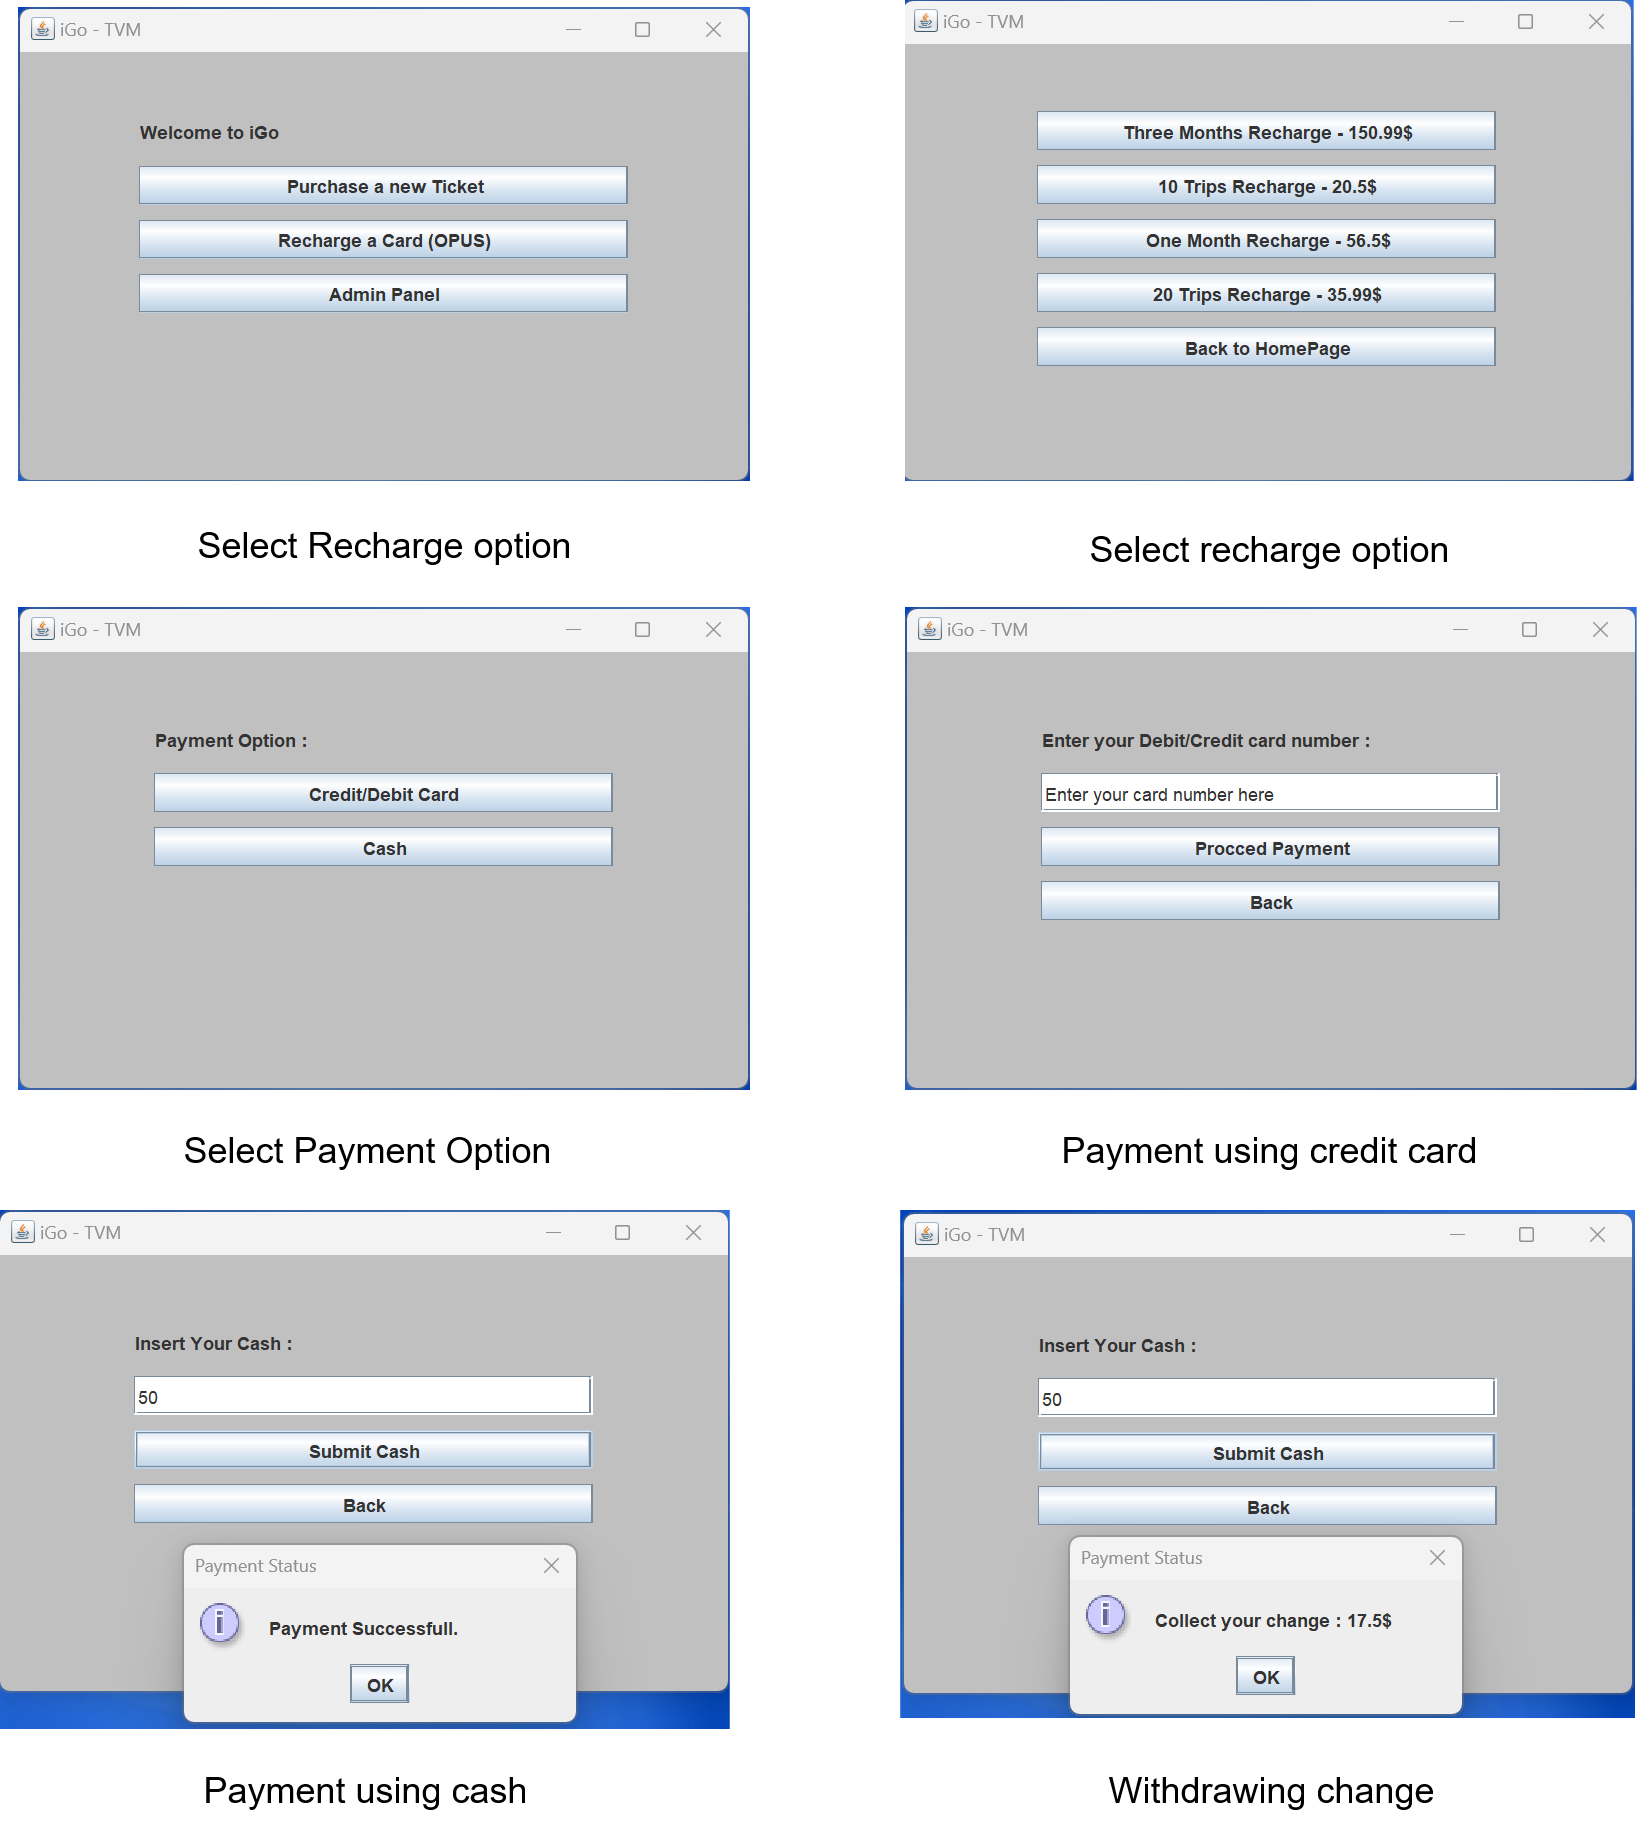
\includegraphics[width=14cm]{3.png} 
\end{figure}
\clearpage
\subsection{Admin Panel}
To access the admin panel, the administrator must select the "Admin Panel" option located on the homepage. Afterward, the administrator must verify their identity by entering the correct password to complete the authorization process. Once authorization is successful, the administrator can proceed to modify the existing ticket plans or recharge plans as required. This will involve entering the updated price for the chosen plan. Once the prices have been successfully updated, a message will be displayed confirming the same.\\
\begin{figure}[h]
\centering
   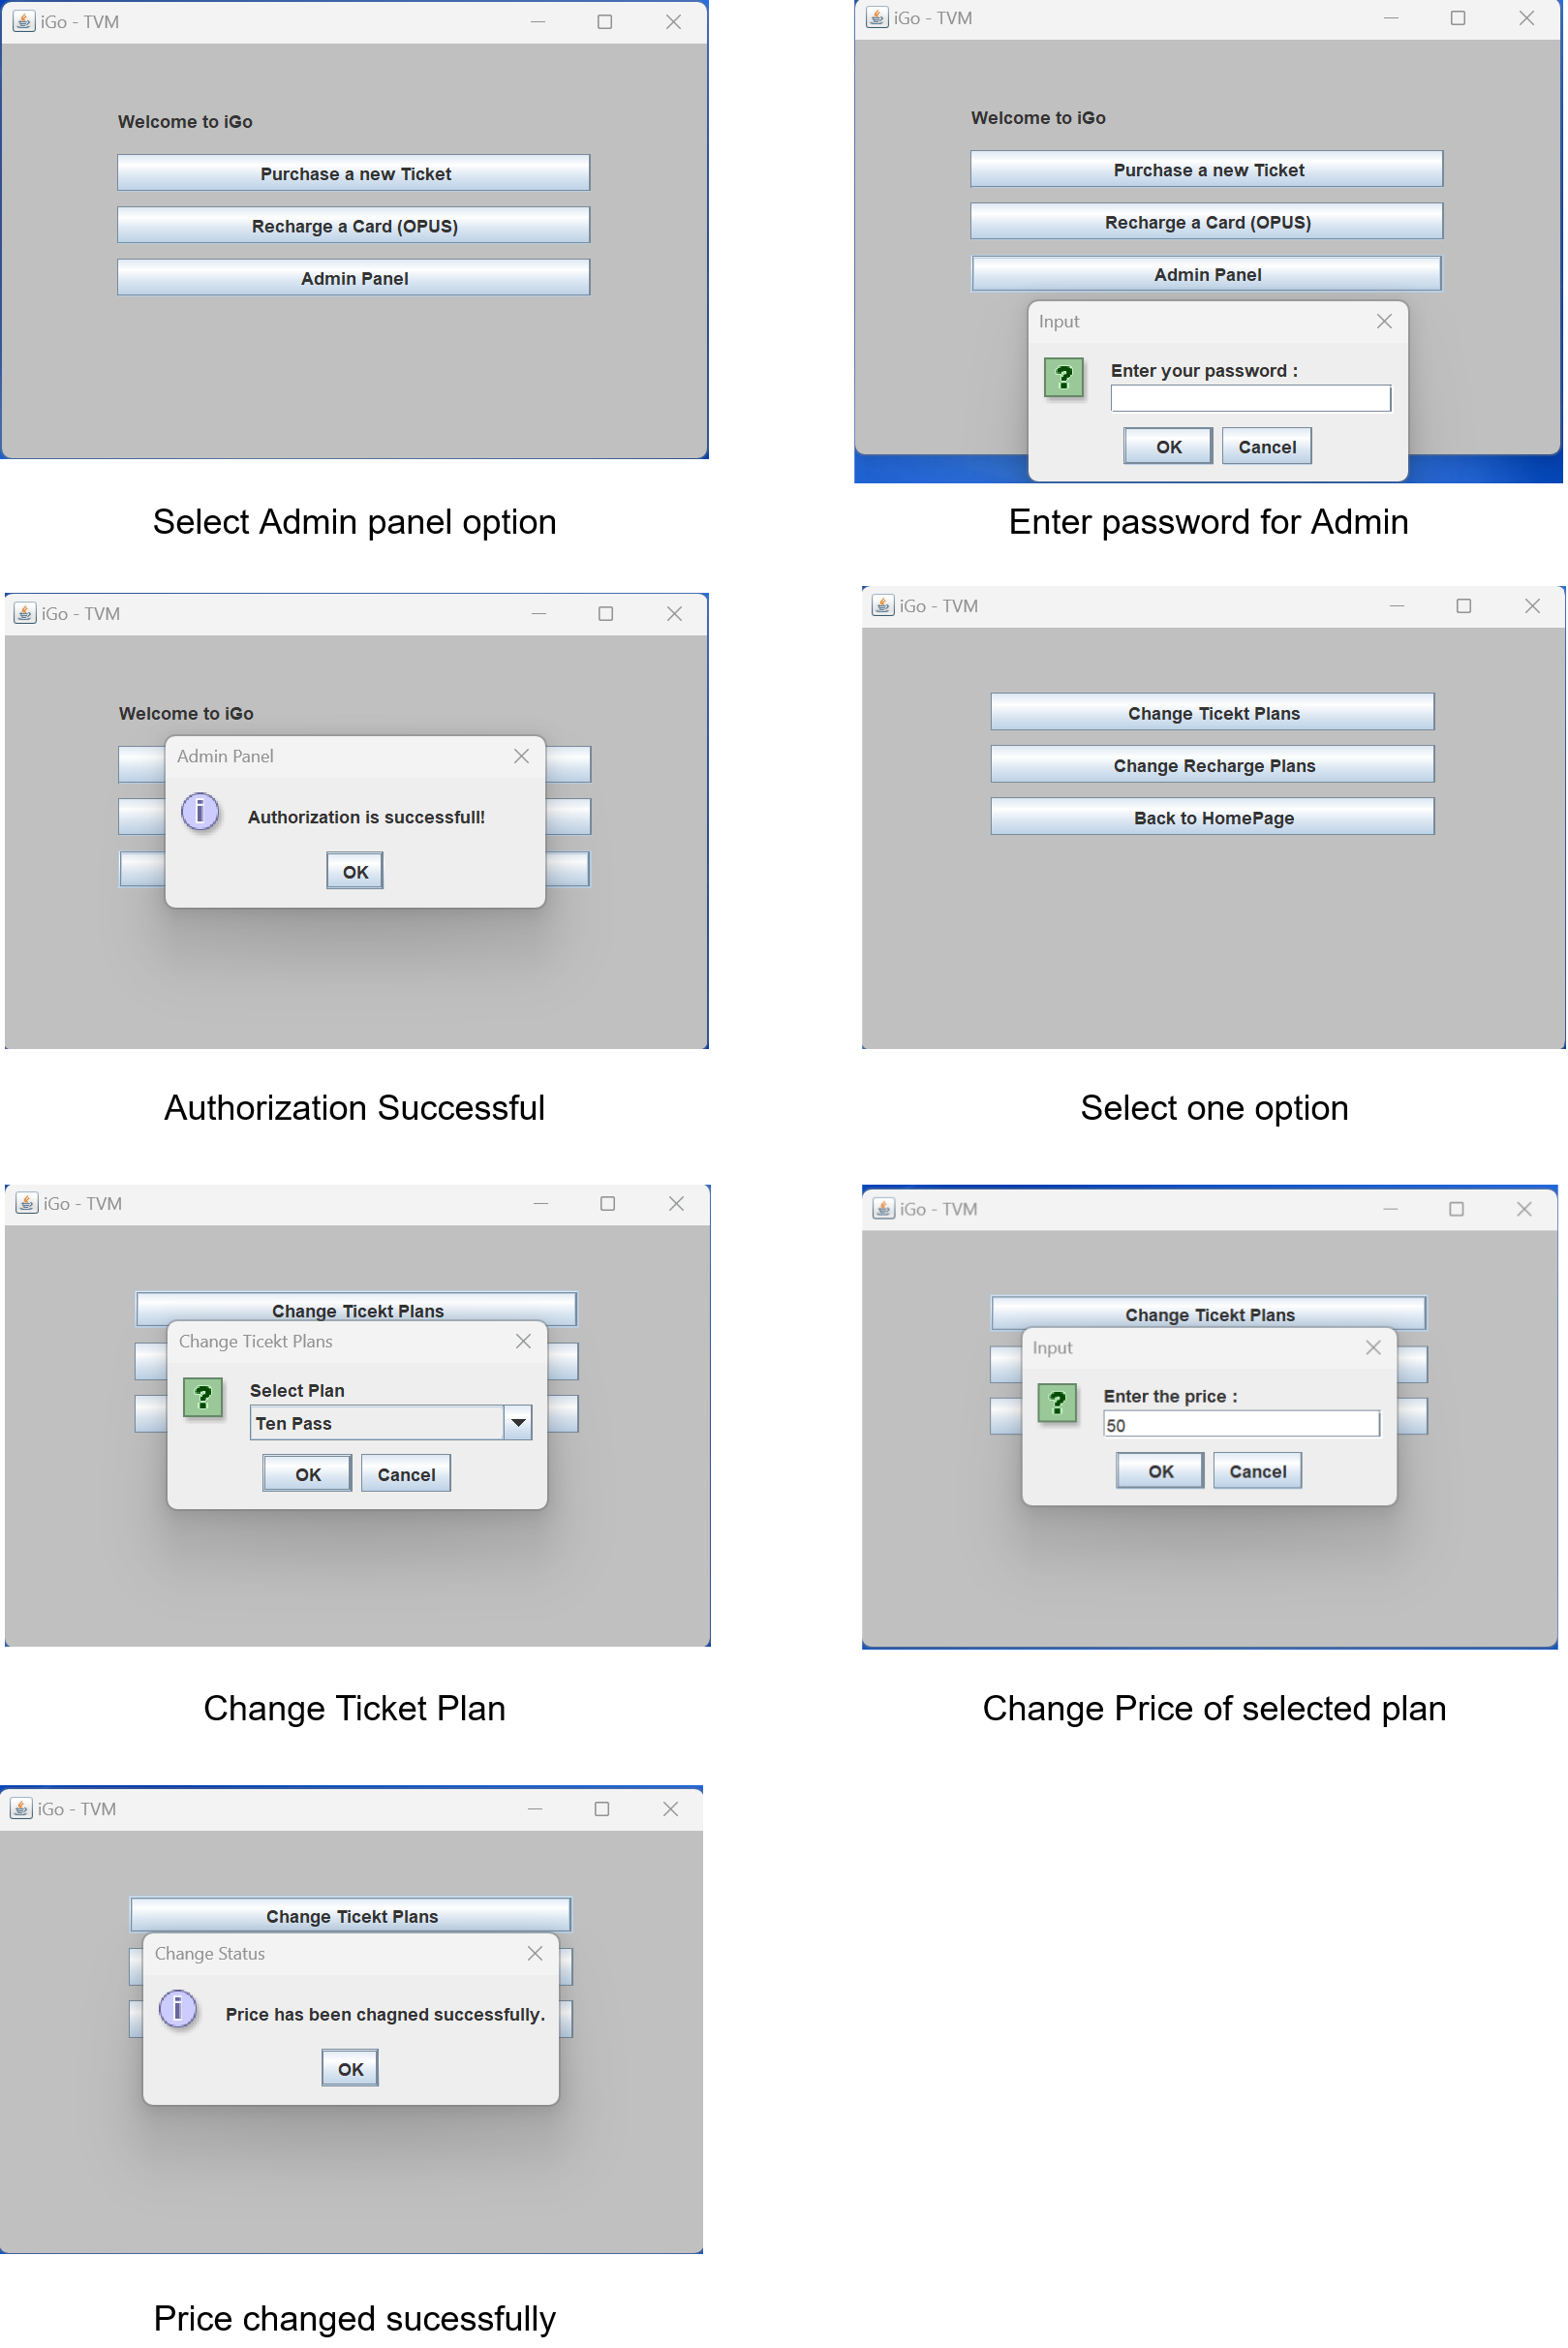
\includegraphics[width=12cm]{5.png} 
\end{figure}
\clearpage
\subsection{Negative Test Cases}
In the case of negative use cases, if the user attempts to enter non-numeric values when inserting the cash amount, a message will be displayed indicating that payment has been denied and prompting the user to enter a valid cash amount. Similarly, for card payments, the inputted card details must be numeric and correct for the payment to be successful. If the email address provided is not in the proper format, the iGO system will not accept it, and the user will be prompted to enter a valid email address. For admin authorization, the password is case sensitive, and any deviation from the correct password format will result in a failed login attempt. Therefore, the administrator must enter the exact password to complete the authorization process successfully.\\
\begin{figure}[h]
\centering
   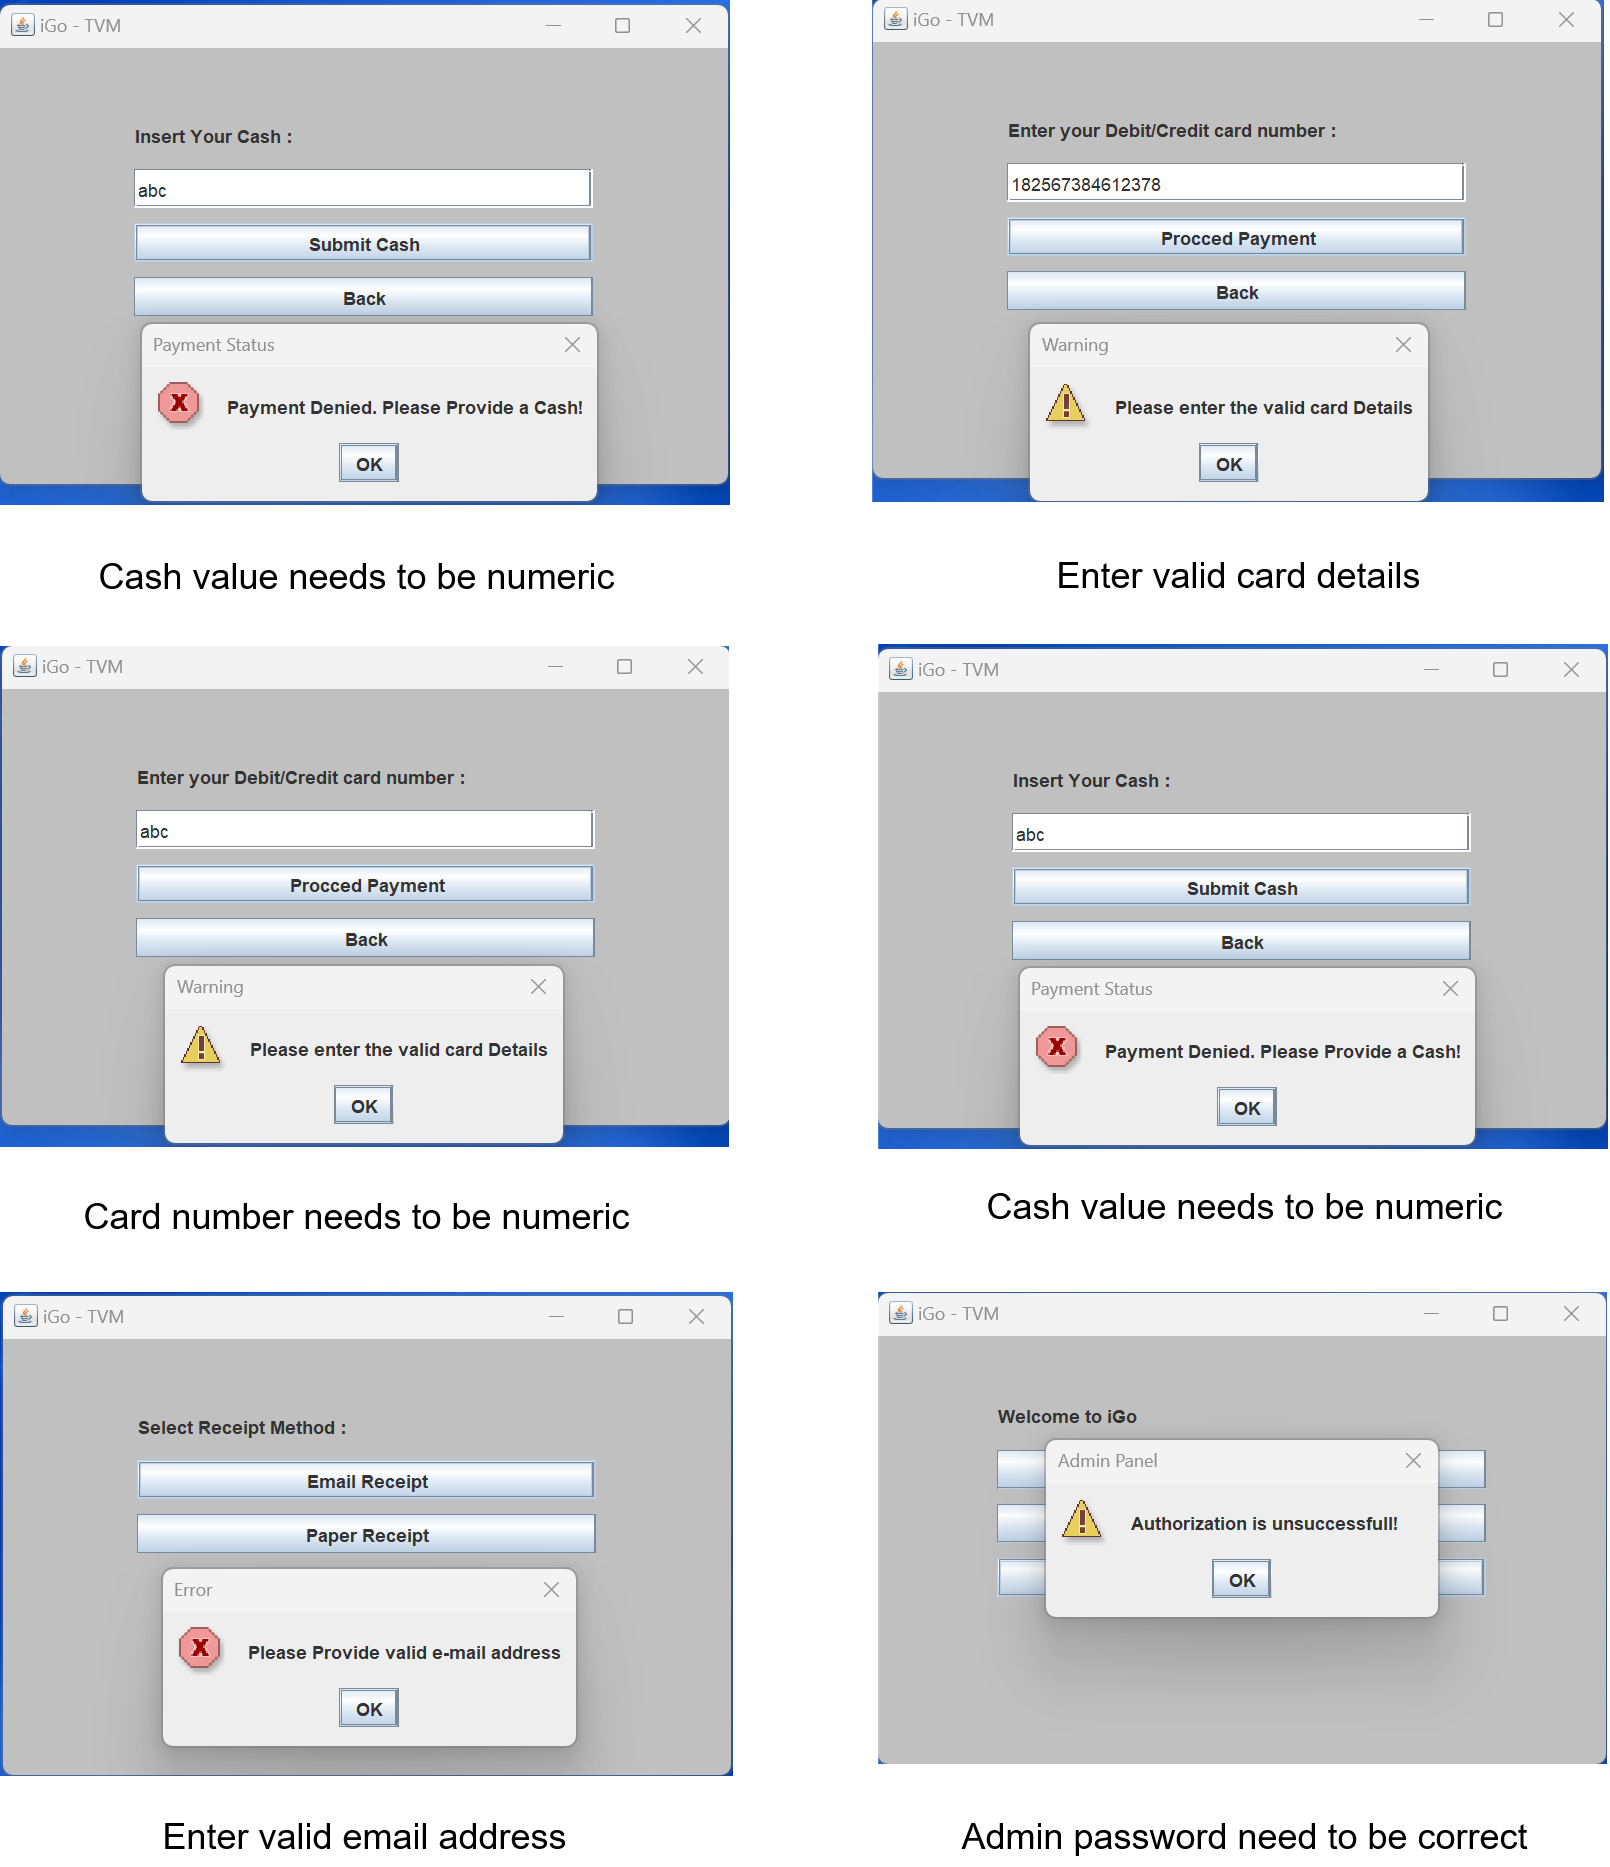
\includegraphics[width=14cm]{6.png} 
\end{figure}

\chapter{Tools Used}
 \begin{itemize}
     \item Overleaf
     \item Xmind
     \item LucidChart
     \item GitHub
     \item Google drive
 \end{itemize}
\chapter{References}
\begin{enumerate}
  \item PANKAJ KAMTHAN (2023) “Introduction to Responsibility-Driven Design "
  \item PANKAJ KAMTHAN (2023) “Introduction to Diagramming"
  \item PANKAJ KAMTHAN (2023) “A Case Study of the Object-Oriented Design of an Elevator Control System”
  \item PANKAJ KAMTHAN (2023) “Introduction To Domain Modeling”
  \item PANKAJ KAMTHAN (2023) “Introduction To Use Case Modeling” 
  \item \url{https://www.lucidchart.com/pages/uml-activity-diagram}
  \item \url{https://echeung.me/crcmaker/}
  \item \url{http://www.stm.info/en}
\end{enumerate}
\end{document}